\documentclass[11pt]{report}
\usepackage[utf8]{inputenc}
\usepackage{graphicx}
\graphicspath{ {images/} }
\usepackage{caption}
\usepackage{subcaption}
\usepackage{float}
\usepackage[width=155mm,top=35mm,bottom=25mm, left=60,bindingoffset=6mm]{geometry}
\usepackage{fancyhdr}
\usepackage{setspace}
\usepackage{verbatim}
\pagestyle{fancyplain}% <- use fancyplain instead fancy
\fancyhf{}
\fancyhead[R]{\thepage}
\renewcommand{\headrulewidth}{0pt}
\setlength{\headheight}{14pt}
\usepackage[hyperfootnotes=false]{hyperref}
\usepackage[style=authoryear,sorting=none]{biblatex}
\addbibresource{references.bib}

\title{Analysis of the variability properties of the stars in the PLATO Input Catalogue}
\author{Adriana Barbieri}
\date{21 June 2023}

\begin{document}
\pagenumbering{roman} 

\begin{titlepage}
%\vspace{3mm}
\begin{figure}[hbtp]
\centering

\includegraphics[scale=.07]{unipd.jpg}
\end{figure}
%\vspace{3mm}
\begin{center}
{{\Large{\textsc{\bf UNIVERSIT\`A DEGLI STUDI DI PADOVA}}}\\}
\vspace{8mm}
%{{\huge{\textsc{\bf PADOVA}}}\\}
%\vspace{8mm}
{\Large{Dipartimento di Fisica e Astronomia ``Galileo Galilei''}} \\
\vspace{3mm}
{\Large{{Master Degree in Astrophysics and Cosmology}}}\\
\vspace{10mm}
{\Large{{Final dissertation}}}\\
\vspace{10mm}
\begin{spacing}{2}
{\LARGE \textbf{Analysis of the variability properties of the stars in the PLATO Input Catalogue}}\\
%\vspace{-5mm}
\end{spacing}
%\vspace{8mm}
\end{center}
\vspace{10mm}
\begin{spacing}{2}
\begin{tabular}{ l  c  c c c  cc c c c l }
{\large{Thesis supervisor}} &&&&&&&&&& {\large{Candidate}}\\
{\large{Prof. Giampaolo Piotto}} &&&&&&&&&& {\large{Adriana Barbieri}}\\
{\large{Thesis co-supervisor}}\\
{\large{Dr. Marco Montalto}}\\
{\large{Thesis external examiner}}\\
{\large{Dr. Silvano Desidera}}\\
\end{tabular}
\end{spacing}
\vspace{8 mm}

\begin{center}
{\Large{19/07/2023}}\\
\vspace{3mm}
{\Large{Academic Year 2022/2023}}
\end{center}
\end{titlepage}
%\clearpage{\pagestyle{empty}\cleardoublepage}



\fancyhf{} % clear all header and footer fields
\fancyhead[RO,R]{\thepage} %RO=right odd, RE=right even
\renewcommand{\headrulewidth}{0pt}

\begin{center}
    \Large
    \textbf{Analysis of the variability properties of the stars in the PLATO Input Catalogue}
    
    \vspace{0.4cm}
    \textbf{Adriana Barbieri}
    
    \vspace{0.9cm}
    \textbf{Abstract}
\end{center}
This thesis work examines the variability properties of a sample of stars included in the PLATO Input Catalogue, which has been selected through a cross-match operation with the variable sources in the Gaia Data Release 3.
Particularly, the study focuses on the photometric, astrometric and spectroscopic data analysis of 11 specific classes of variable objects, and on the relevance of these sources for the PLATO space mission.\\
Finally, a comparison with several catalogues of variable objects from the literature is undertaken. 

\chapter*{Dedication}

%To mum and dad

%\chapter*{Declaration}

%I declare that..

\chapter*{Acknowledgements}

%I want to thank...

%Supported by grant numbers...

This work has made use of data from the European Space Agency (ESA) mission {\it Gaia} %(\url{https://www.cosmos.esa.int/gaia}), 
processed by the {\it Gaia} Data Processing and Analysis Consortium (DPAC,
\url{https://www.cosmos.esa.int/web/gaia/dpac/consortium}). Funding for the DPAC
has been provided by national institutions, in particular the institutions
participating in the {\it Gaia} Multilateral Agreement.\\
The Gaia mission website is \url{https://www.cosmos.esa.int/gaia}, the Gaia archive website is \url{https://archives.esac.esa.int/gaia}.\\
Some of the data presented in this work were obtained from the Mikulski Archive for Space Telescopes (MAST) at the Space Telescope Science Institute.  STScI is operated by the Association of Universities for Research in Astronomy, Inc., under NASA contract NAS5–26555. Support to MAST for these data is provided by the NASA Office of Space Science via grant NAG5–7584 and by other grants and contracts.\\
The All-sky PLATO Input Catalogue (asPIC) can be accessed via \url{https://doi.org/10.17909/t9-8msm-xh08}.

\tableofcontents


\listoffigures


\listoftables

\doublespacing
\chapter*{Introduction}

\pagenumbering{arabic} 
\chapter{PLATO space mission}
\section{Mission overview}



\subsection{Scientific objectives}
\subsection{Instrumentation and payload}  
\subsection{Mission design}
\section{PLATO Input Catalogue}
\parencite{Montalto_2021}
\section{Long-duration Observation Phase field selection}

\parencite{Nascimbeni_2022}

\section{PLATO Roadmap and legacy}

\chapter{Gaia space mission}


\section{Mission overview}


\parencite{2016}

\subsection{Scientific objectives}



\subsection{Instrumentation and payload}  
\subsection{Mission design}
\section{Gaia Data Release 3}
\parencite{https://doi.org/10.48550/arxiv.2208.00211}
\section{Variability and Specific Object Studies modules}

%Variability analysis can be defined as the comprehensive assessment of the degree and character of patterns of variation over time intervals.

As stated in \cite{Rimoldini}, time-dependent brightness variations of celestial objects may
be caused by different phenomena, and a certain set of
classes can be identified to describe different variability types.
Indeed Gaia offers the unique opportunity to study variability of close to 2 billion objects: its
%thanks to the multiband G, G BP , G RP photometric time series, but also to the other spectrophotometric and RVS time series.
multi-epoch observations and sparse sampling allow for the
detection of periodic signals ranging from minutes to years and
for medium to long-term non-periodic variability.
%The Gaia DR3 photometric time series provided sufficient information to classify ten million variable objects into two dozen variability class groups across the whole sky
%\parencite{Rimoldini}
% for this variability analysis: astrometry, photometry, spectroscopy (epoch radial velocity). I also used some astrophysical parameters

Among the strong points of the mission for variability analysis, we can mention, in addition to its well-known astrometric
capabilities, the large dynamical range reached in stellar brightness, from a few magnitudes to fainter than 20 mag, the specific scanning law leading to irregularly sampled time series,
and the quasi-simultaneity (within tens of seconds) of the observations in G photometry, $G_{BP}$ and $G_{RP}$ spectrophotometry, and
RVS (Radial Velocity Spectrometer) spectroscopy.





\begin{comment}
filtered magnitude time series in G FoV (i.e. averaging the G CCD
measurements within one FoV transit), G BP , and G RP as
described in Eyer et al. (2017) and in Holl et al. (2018)
\end{comment}


% flux variations, variations in brightness
% The structure function characterizes light curve variability by quantifying the change in amplitude Δmij as a function of time lag Δtij between observations at epochs i and j. Following the prescription of Schmidt et al. (2010), variability structure function of the source magnitude
% Parameters γ and Ar of the variability structure function for the stellar (blue points) and quasar (red points) test samples. Large A’s indicate large fluctuation amplitudes. Large γ’s indicate an increase of the fluctuation amplitude with time.
% method that characterizes light curve variability

\section{Gaia Roadmap and legacy}





\chapter{Variability analysis}
\section{Preliminary data analysis}


Variability analysis can be defined as the comprehensive assessment of the degree and character of patterns of variation of the source's brightness over time intervals. % astrophysical context
% A time series generally has these three components: a trend, seasonality, and noise. 

% pic targets from prof (asPIC1.1 contains 2 675 539 stars.)
In this thesis work I analyzed two sample of stars  obtained from the two outer regions centered on the Long-duration Observation Phase (LOP) north and south fields in the PLATO Input Catalogue, selected as explained in \cite{Nascimbeni_2022}.

%cross matching each lop with each variability class from gaia dr3
These outer caps count respectively 543394 and 593563 targets, that have been cross-matched by the unique source identifier $\textit{source\_id}$ with each variable source of the 11 Specific Object Studies (SOS) modules in Gaia Data Release 3.\\
As described in \cite{Eyer} and section 2, these variability classes include RR Lyrae stars, Cepheids, eclipsing binaries, upper Main Sequence oscillators, solar-like variables with rotational modulation, short timescale variables, long period variables, active galactic nuclei, microlensing events, compact companions
%black hole, a neutron star or a white dwarf
and stellar hosts of transiting extra-solar planets.

%arrange tables with astrophysical parameters from gaia dr3 
Following the cross-matching operation, the resulting non-null variability classes have been complemented with selected photometric, spectroscopic, astrometric and astrophysical parameters of the sources, obtained via ADQL (Astronomical Data Query Language) Advanced Search in the Gaia Archive query interface.
	



%download from archive epoch photometry and RV for each class
Non tabular data such as epoch photometry in the G, $G_{BP}$ , and $G_{RP}$ bands and mean spectra
%and epoch radial velocities 
have instead been extracted via DataLink from the Gaia Archive.

%plot aitoff projection, de reddened absolute cmd
The outcome of this preliminary analysis is the distribution of several classes of variable objects in the all-sky PLATO Input Catalogue that is reported in table \ref{tab:pic1_2}.

\begin{table}
\centering
\begin{tabular}{c c c}
    \hline
    \hline
    Variability class & LOPN1 & LOPS2 \\
     \hline
    Short timescale & 2996 & 4081 \\
    Eclipsing binaries & 2977 & 3467 \\
    Solar-like & 1794 & 1849 \\
    MS oscillators & 153 & 438 \\
    RR Lyrae & 84 & 78 \\
    Exoplanetary hosts & 21 & 31 \\
    Cepheids & 1 & 0 \\
    Long period & 0 & 1 \\
    \hline
\end{tabular}
\caption{Variable sources in the PIC outer LOP fields.}
\label{tab:pic1_2}
\end{table}

%From this preliminary analysis, this distribution has been obtained for the variable sources in the all-sky PLATO Input Catalogue: the northern outer LOP region hosts 2996 short timescale variables, 2977 eclipsing binaries, 1794 solar-like variables presenting rotational modulation, 153 MS oscillators, 84 RR Lyrae stars, 21 transiting planets hosts and one Cepheid star, while the southern outer LOP field hosts 4081 short timescale variables, 3467 eclipsing binaries, 1849 solar-like stars, 438 MS oscillators, 78 RR Lyrae stars, 31 planet hosts and one long period variable.
No Active Galactic Nuclei, microlensing events and compact companions are collected in the PLATO Input Catalogue.


The main parameters selected for each of the aforementioned classes of variable objects have been collected in Tables \ref{tab:week1} and \ref{tab:week2}.

The all-sky distribution of the different classes of variable sources in Aitoff projection and Galactic coordinates is displayed in
Figure \ref{fig:All-sky map}, while the absolute Color-Magnitude Diagrams corrected for extinction are shown in \ref{fig:aCMD}.\\
%\ref{fig:LOPN1} and \ref{fig:LOPS2}

For each variability class, sky map distributions, %absolute color-magnitude diagrams 
observational Hertzsprung–Russell diagrams, and photometric time series have been obtained.

Moreover in order to characterize variability the statistics of photometric time series have been exploited, such as the Abbe value and the skewness magnitude for G FoV transits, that together constitude a metric targeting non-periodic variations.
The Abbe value, or von-Neumann ratio statistic, measures the point-to-point scatter in a photometric time series, and is an estimate of the regularity of the light curve variability pattern over the duration of the observations; in other words it estimates the smoothness of the light curve. The skewness of the magnitude distribution is instead a measure of the asymmetry of the light curve.
A metric targeting periodic variations is given by the distribution of the ratio of the two bands mean photometric uncertainties as a function of the median magnitude in the G band,
where stellar pulsations are expected to exhibit larger variations in the $G_{BP}$ than in the $G_{RP}$ band.

% other methods to characterizes light curve variability
% - time series standard deviation as a function of magnitude
% (the standard deviation is a measure of the amount of variation or dispersion of a set of values.)

In the following sections the main properties of the variable sources located in the northern and southern outer LOP fields are investigated.






%\newpage

\begin{table}[H]
    \begin{subtable}[h]{1.15\textwidth}
        \centering
       \small
 \resizebox{\textwidth}{!}{        
\begin{tabular}{ccccc}
\cline{2-5}
                                              & \multicolumn{4}{c}{\textbf{Variability types}}                                                                                                                                                                                                                        \\ \hline \hline
\multicolumn{1}{l|}{\textbf{gaiadr3. tables}}          & \textbf{RR Lyrae} 
 & \textbf{Cepheids} 
& \textbf{planetary transits}                                                                  & \textbf{eclipsing binaries}       \\ \hline
\multicolumn{1}{l|}{gaia\_source}             & l    &l                                                                              & l                                                                                  &                                l                    \\
\multicolumn{1}{l|}{gaia\_source}             & b         &b                                                                         & b                                                                                  &                                b                         \\
\multicolumn{1}{l|}{gaia\_source}             & parallax                                                                           & parallax                                                                           &                                parallax           &  parallax                                          \\

\multicolumn{1}{l|}{vari\_summary}            & median\_mag\_g\_fov                                                                & median\_mag\_g\_fov                                                                &       median\_mag\_g\_fov      &  median\_mag\_g\_fov                                                                \\
\multicolumn{1}{l|}{vari\_summary}            & median\_mag\_bp                                                                    & median\_mag\_bp                                                                    &      median\_mag\_bp     &      median\_mag\_bp                                                                          \\
\multicolumn{1}{l|}{vari\_summary}            & median\_mag\_rp                                                                    & median\_mag\_rp                                                                    &       median\_mag\_rp       & median\_mag\_rp                                                                \\
\multicolumn{1}{l|}{astrophysical\_parameters} &                ag\_gspphot &                   &     ag\_gspphot                &                                ag\_gspphot                             \\
\multicolumn{1}{l|}{vari\_type}               & source\_id    & source\_id                                                                     & source\_id                                                                                               &   source\_id                                                         \\
\multicolumn{1}{l|}{vari\_type}               & p\_f     & p\_f                                                                          & transit\_period                                                                               & frequency      \\
\multicolumn{1}{l|}{vari\_type}               &    p1\_o     & p1\_o                                                                          &      &          \\
\multicolumn{1}{l|}{vari\_type}               & peak\_to\_peak\_g     &                                                             &                                                                 &            \\
\multicolumn{1}{l|}{vari\_type}               & metallicity   &                                                                     &                                                                        &                    \\
\multicolumn{1}{l|}{vari\_type}     & best\_classification & type\_best\_classification &  &  \\
\multicolumn{1}{l|}{vari\_type}     & reference\_time\_g & reference\_time\_g  & transit\_reference\_time   &               reference\_time     \\
\multicolumn{1}{l|}{vari\_type}     & reference\_time\_bp & reference\_time\_bp  &  &  \\
\multicolumn{1}{l|}{vari\_type}     & reference\_time\_rp & reference\_time\_rp  &  &  \\
\multicolumn{1}{l|}{vari\_type}     & reference\_time\_rv &   &  &  \\
\multicolumn{1}{l|}{datalink}                 & \begin{tabular}[c]{@{}c@{}}epoch photometry\\ (G, BP, RP time series)\end{tabular} & \begin{tabular}[c]{@{}c@{}}epoch photometry\\ (G, BP, RP time series)\end{tabular} &  \begin{tabular}[c]{@{}c@{}}epoch photometry\\ (G, BP, RP time series)\end{tabular}   &  \begin{tabular}[c]{@{}c@{}}epoch photometry\\ (G, BP, RP time series)\end{tabular}                                                          \\
\multicolumn{1}{l|}{vari\_epoch\_radial\_velocity}    &   rv\_obs\_time         &                                                                        &                                                                                    &                                                                 \\ 
\multicolumn{1}{l|}{vari\_epoch\_radial\_velocity}    &   radial\_velocity         &                                                                        &                                                                                    &                                                                 \\ 
\multicolumn{1}{l|}{vari\_epoch\_radial\_velocity}    &   radial\_velocity\_error         &                                                                        &                                                                                    &                                                                 \\ 
\hline
\end{tabular}
}
       \caption{}
       \label{tab:week1}
    \end{subtable}
    \hfill \\ \\ \\
    \begin{subtable}[h]{1.15\textwidth}
        \centering
       \small
\resizebox{\textwidth}{!}{  
\begin{tabular}{ccccc}
\cline{2-5} 
	& \multicolumn{4}{c}{\textbf{Variability types}}           
\\ \hline   \hline                                                                                                                             
\multicolumn{1}{l|}{\textbf{gaiadr3. tables}}           & \textbf{rotation modulation}       & \textbf{MS oscillator} & \textbf{short timescale}    & \textbf{long period}  \\ \hline
\multicolumn{1}{l|}{gaia\_source}              &         l                           &         l               &           l                  &         l                                                 \\
\multicolumn{1}{l|}{gaia\_source}              &          b                          &           b             &           b                  &                    b                                     \\
\multicolumn{1}{l|}{gaia\_source}              &     parallax                                 &    parallax                    &        parallax                     &            parallax                              \\
\multicolumn{1}{l|}{vari\_summary}             &            median\_mag\_g\_fov                             &        median\_mag\_g\_fov                 &         median\_mag\_g\_fov                     &                    median\_mag\_g\_fov                                     \\
\multicolumn{1}{l|}{vari\_summary}             &    median\_mag\_bp                                   &     median\_mag\_bp                       &         median\_mag\_bp                        &                                           median\_mag\_bp                      \\
\multicolumn{1}{l|}{vari\_summary }            &          median\_mag\_rp                           &          median\_mag\_rp              &         median\_mag\_rp                    &                                         median\_mag\_rp                 \\

\multicolumn{1}{l|}{astrophysical\_parameters} &                ag\_gspphot                    &     ag\_gspphot                &                                ag\_gspphot           &        ag\_gspphot                                  \\

\multicolumn{1}{l|}{astrophysical\_parameters} &                                    & mg\_gspphot          &                             &                                                            \\
\multicolumn{1}{l|}{astrophysical\_parameters} &                                    & vsini\_esphs            &                             &                                                                  \\
\multicolumn{1}{l|}{vari\_type}                &                 source\_id                        &      source\_id                    &            source\_id                   &        source\_id                                                        \\
\multicolumn{1}{l|}{vari\_type }               & best\_rotation\_period             & frequency1             & frequency           & \multicolumn{1}{c}{frequency}                              \\
\multicolumn{1}{l|}{vari\_type}                & max\_activity\_index\_g            & amplitude\_g\_freq1    & amplitude\_estimate & amplitude                                           \\
\multicolumn{1}{l|}{vari\_type}                & segments\_rotation\_period &                        &                             &                                                                \\
\multicolumn{1}{l|}{vari\_type}                & segments\_start\_time &                        &                             &                                                                \\
\multicolumn{1}{l|}{vari\_type}                & segments\_end\_time &                        &                             &                                                                \\
\multicolumn{1}{l|}{datalink}                  &           \begin{tabular}[c]{@{}c@{}}epoch photometry\\ (G, BP, RP time series)\end{tabular}                          &     \begin{tabular}[c]{@{}c@{}}epoch photometry\\ (G, BP, RP time series)\end{tabular}                     &       \begin{tabular}[c]{@{}c@{}}epoch photometry\\ (G, BP, RP time series)\end{tabular}                        &         \begin{tabular}[c]{@{}c@{}}epoch photometry\\ (G, BP, RP time series)\end{tabular}                                        \\

\hline
\end{tabular}
}
        \caption{}
        \label{tab:week2}
     \end{subtable}
     \caption{Astrometric, photometric, spectroscopic and astrophysical parameters for each GDR3 variability class SOS module in the PLATO Input Catalogue.}
     \label{tab:temps}
\end{table}

\newpage

\begin{figure}[ht]
%\centering
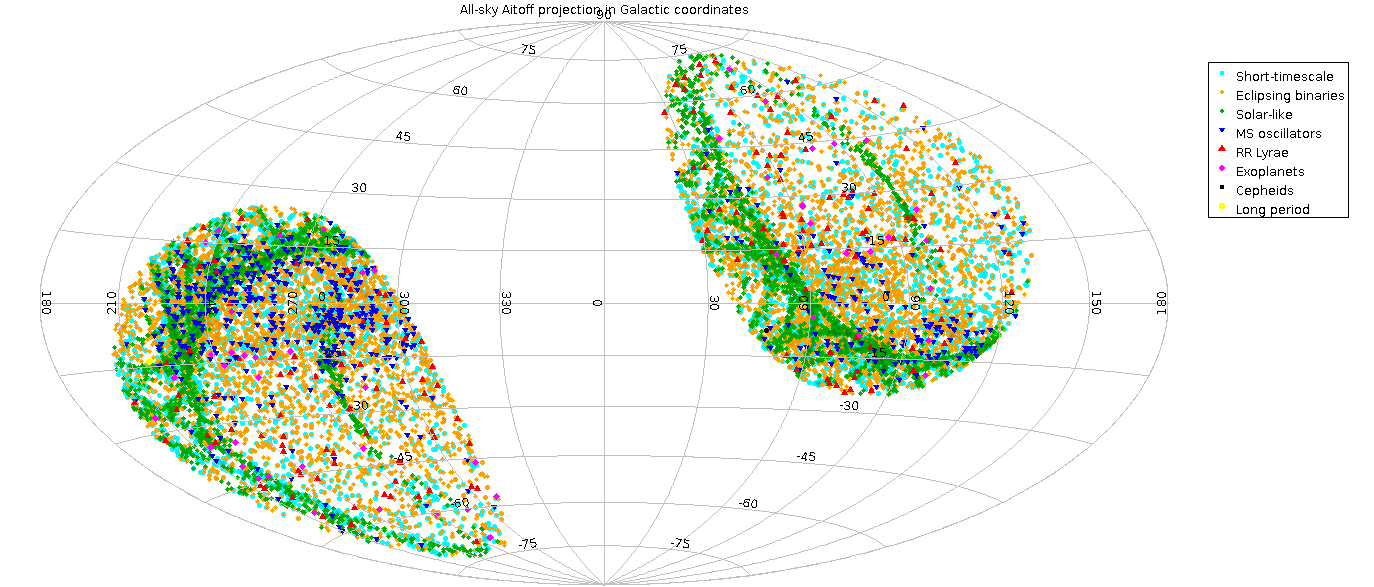
\includegraphics[scale=0.35]{all_aitoff_2.png}
\caption{All-sky distribution of the variable sources in Aitoff projection and Galactic coordinates}
\label{fig:All-sky map}
\end{figure}


\newpage

\begin{figure}[h]
    \centering
        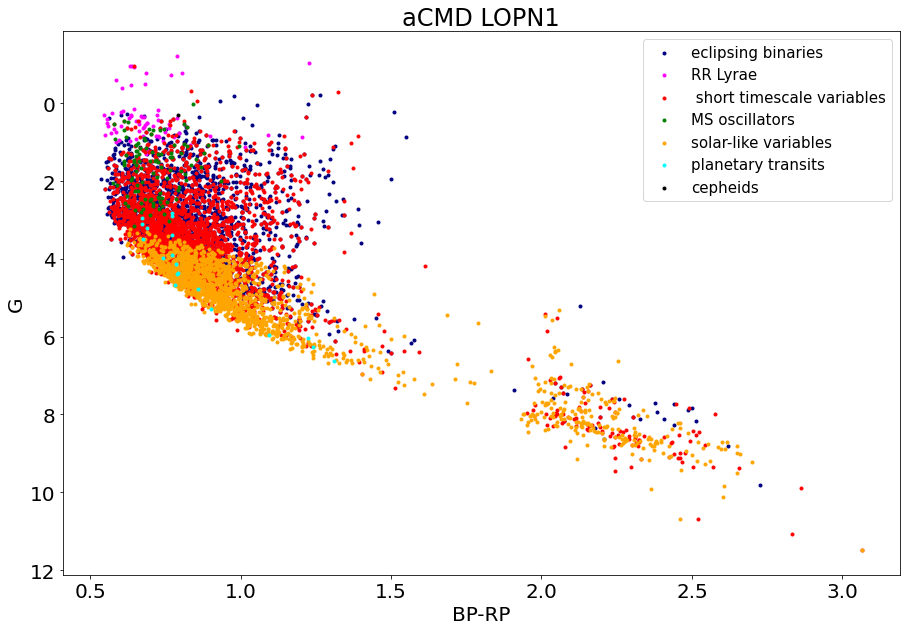
\includegraphics[scale=0.35]{dereddened_aCMD_lopn1.png}
       % \caption{LOPN1}
        \label{fig:LOPN1}
        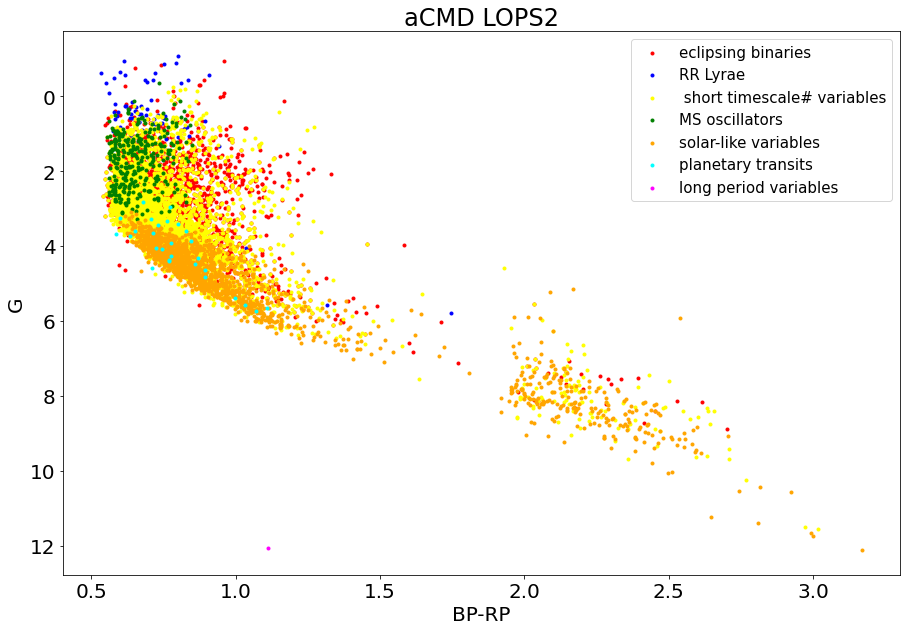
\includegraphics[scale=0.35]{dereddened_aCMD_lops2.png}
      %  \caption{LOPS2}
        \label{fig:LOPS2}
    \caption{Dereddened absolute Color-Magnitude diagrams for both PLATO LOP fields}
    \label{fig:aCMD}
\end{figure}

\newpage

\section{RR Lyrae}
% ages from astrophysical parameters supp table in Gaia Archive
% age distribution, period-amplitude diagram color coded for metallicity (absorption can be derived), lightcurve 
%  RRd source id 4672117758766686720
% p1 to be included in the parameters table

RR Lyrae stars are a class of pulsating stars known to be excellent distance indicators due to the strong correlation between their absolute magnitude and metallicity, and therefore are used as standard candles for measuring (extra-)galactic distances.
They are also regarded as tracers of the chemical and dynamical properties of the oldest observable population of stars, and are typically low mass (M $ \approx$ 0.6-0.8 $\mathrm{M_{\odot}}$), old (ages $>$ 9-10 Gyr) and metal-poor stars whose surface expands
and contracts regularly with periods shorter than a day \parencite{refId4}.\\
RR Lyrae stars can be subclassified into RRab, RRc and RRd depending on their pulsation mode, respectively called fundamental, radial first overtone and double mode (the latter is given by the superposition of the other two ones excited simultaneously).\\
The ab-type RR Lyrae stars oscillate with periods typically between about 0.42 d and 1 d, their light curves look asymmetrical and sawtooth-shaped and present a variation in brightness of up to one magnitude in the \textit{Gaia} visual G band, while c-type RR Lyrae stars have periods between about 0.2 d and 0.42 d, symmetric and almost sinusoidal light curves and brightness variations of up to about half a magnitude in the visual band.\\
The PLATO Input Catalogue features 3 RRc stars and 81 RRab stars in the northern outer LOP field, and one RRd star, 8 RRc stars and 69 RRab stars in the southern outer LOP field. 
In fig. \ref{fig:All-sky map of RR Lyrae stars} the sky map distribution of these periodic pulsating sources can be observed, while fig. \ref{fig:Absolute CMD corrected for extinction for the total RR Lyrae sample in PIC} displays the absolute colour-magnitude diagram corrected for extinction for the RR Lyrae stars of both galactic emispheres.
Fig. \ref{fig:PA} shows the P-A diagram of the pulsation period and the peak to peak amplitude of the light variation in the G band for the total considered sample of RR Lyrae stars, where the sources have been colour-coded according to their metallicity; it appears that the sources with a longer period present lower values of metal abundance.
From figure \ref{fig:metrics} (top) it appears that the mean of the magnitude skewness distribution is negative, as it is to be expected for a sample mostly composed of ab-type RR Lyrae stars, whose lightcurves are asymmetrical.
The periodic pulsating nature of RR Lyrae can be inferred also from \ref{fig:metrics} (bottom), that shows the ratio of the two bands variances to be almost constant as a function of the median magnitude per FoV in the G band, with an abrupt increase towards fainter magnitudes probably caused by a noise saturation\\
The lightcurves of two arbitrary RR Lyrae stars from our sample are collected in figures \ref{fig:lightcurve_rrab_f} and \ref{fig:lightcurve_rrc_f}, where the typical saw-tooth shape of the RRab class and sinusoidal shape of the RRc class can be respectively observed.
The radial velocity time series of the sources RRab Gaia DR3 2926381228470699392 and RRc Gaia DR3 1956531880222667904 are displayed in figures \ref{fig:rv_rrab} and \ref{fig:rv_rrc}.


\begin{figure}[H]
\centering
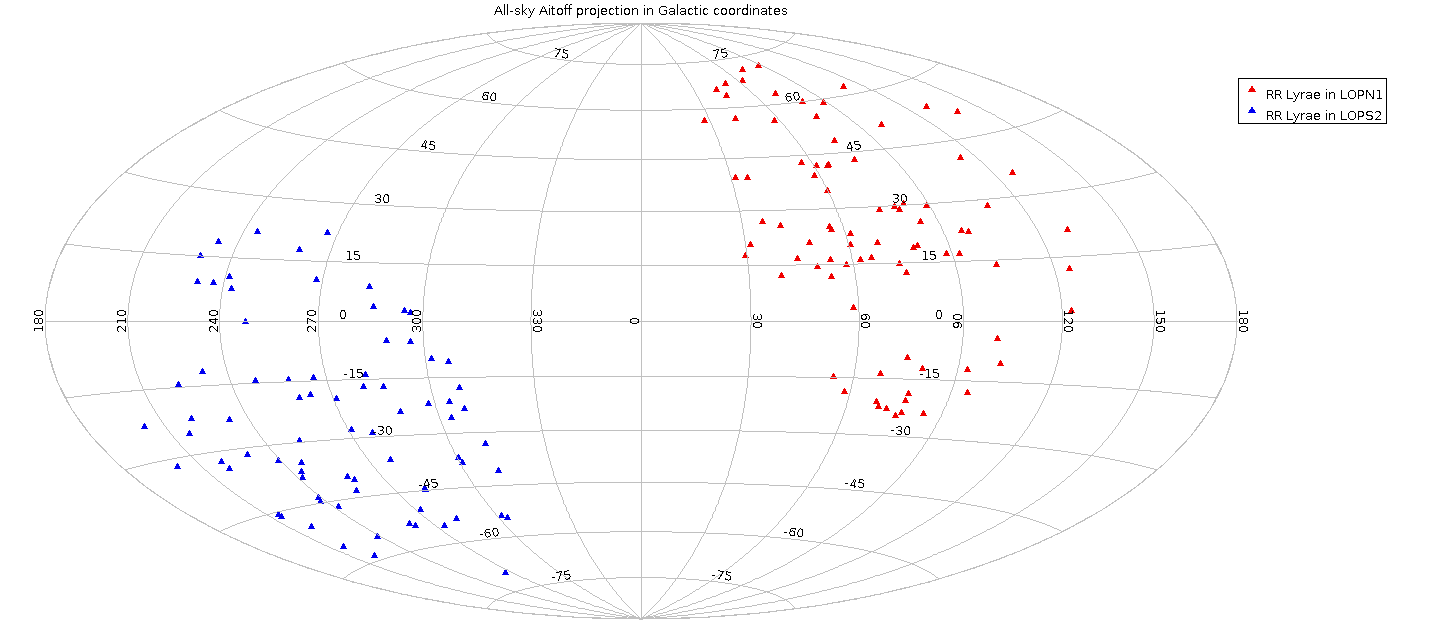
\includegraphics[scale=0.35]{RR_aitoff.png}
\caption{Sky map of RR Lyrae stars in Galactic coordinates }
\label{fig:All-sky map of RR Lyrae stars}
\end{figure}

\begin{comment}
\begin{figure}[H]
\centering
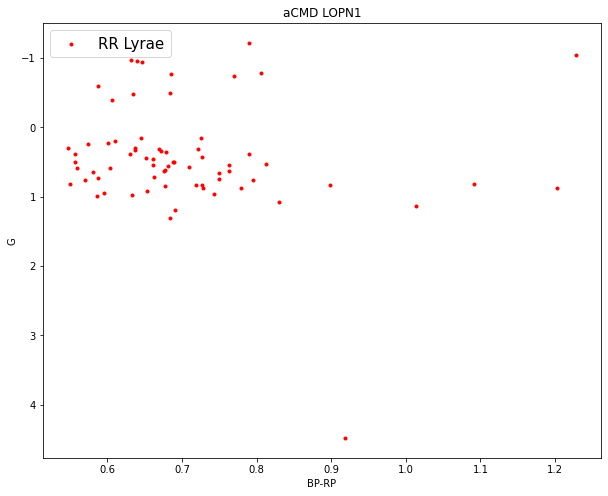
\includegraphics[scale=0.5]{rr_cmd.png}
\caption{Absolute CMD corrected for extinction for the RR Lyrae stars in LOPN1}
\label{fig:Absolute CMD corrected for extinction for the RR Lyrae stars in LOPN1}
\end{figure}

\begin{figure}[H]
\centering
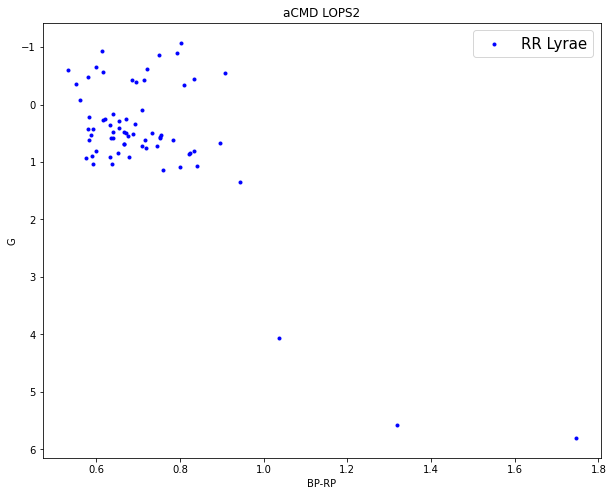
\includegraphics[scale=0.5]{rr2_cmd.png}
\caption{Absolute CMD corrected for extinction for the RR Lyrae stars in LOPS2}
\label{fig:Absolute CMD corrected for extinction for the RR Lyrae stars in LOPS2}
\end{figure}
\end{comment}

\begin{figure}[H]
\centering
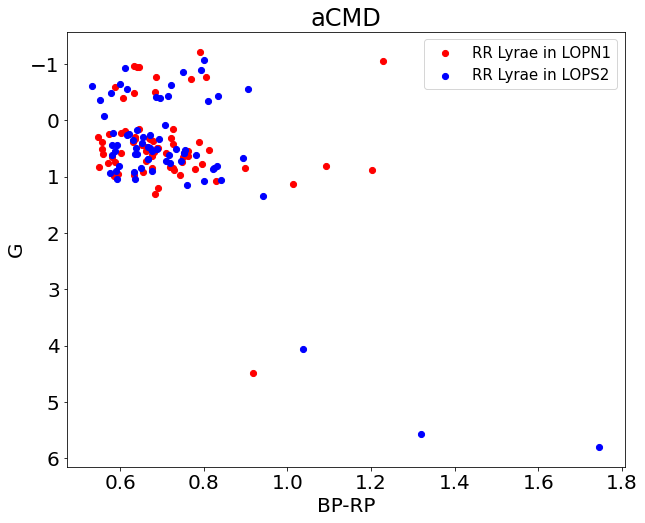
\includegraphics[scale=0.5]{rr_acmd.png}
\caption{Absolute CMD corrected for extinction for the total RR Lyrae sample in PIC}
\label{fig:Absolute CMD corrected for extinction for the total RR Lyrae sample in PIC}
\end{figure}


\begin{figure}[H]
\centering
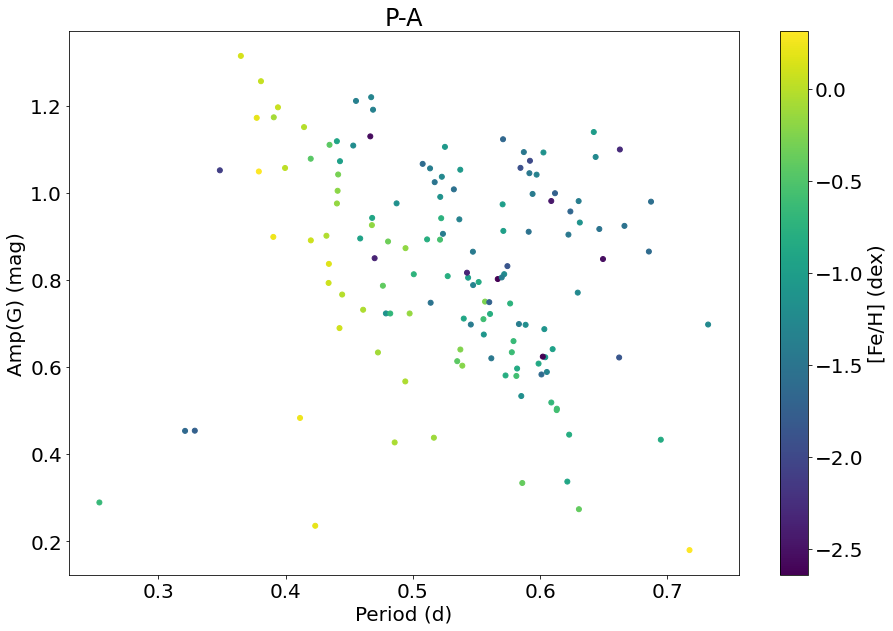
\includegraphics[scale=0.5]{metal.png}
\caption{Period - Amplitude diagram for RR Lyrae stars colour-coded according to their metallicity}
\label{fig:PA}
\end{figure}

\begin{figure}[H]
\centering
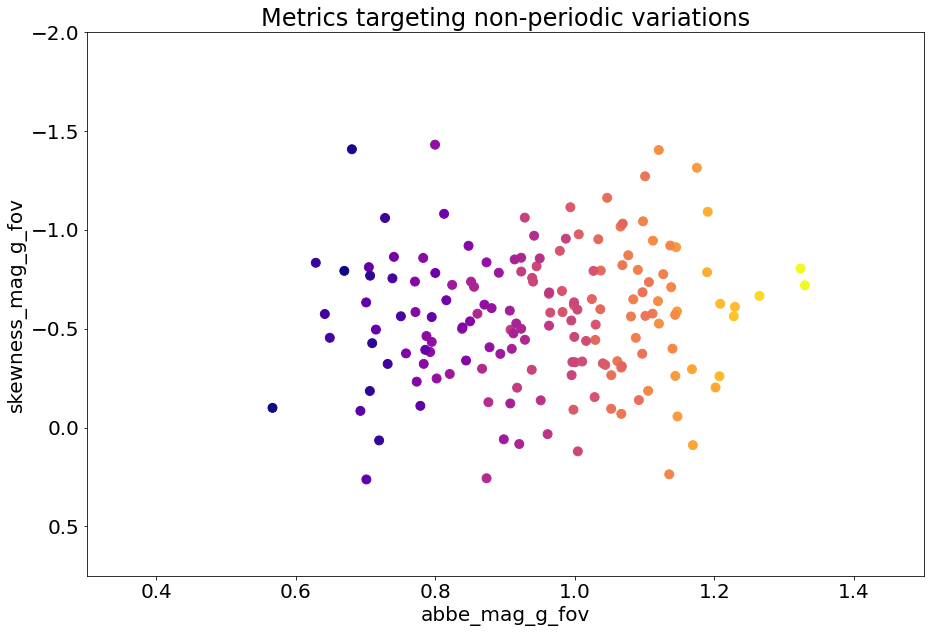
\includegraphics[scale=0.35]{abbe.png}
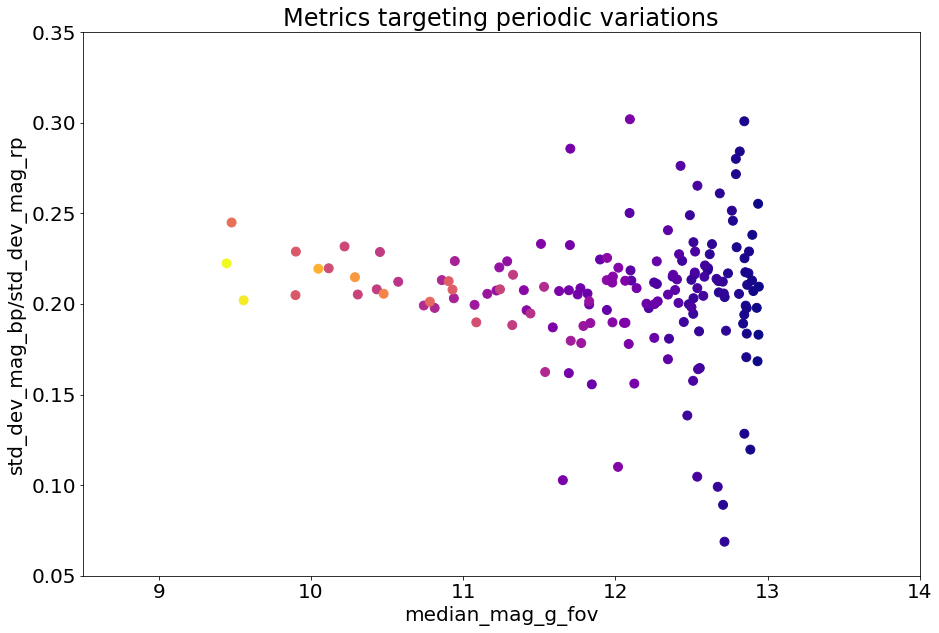
\includegraphics[scale=0.35]{std.png}
\caption{Metrics targeting non-periodic (top) and periodic (bottom) variations}
\label{fig:metrics}
\end{figure}

\begin{figure}[H]
\centering
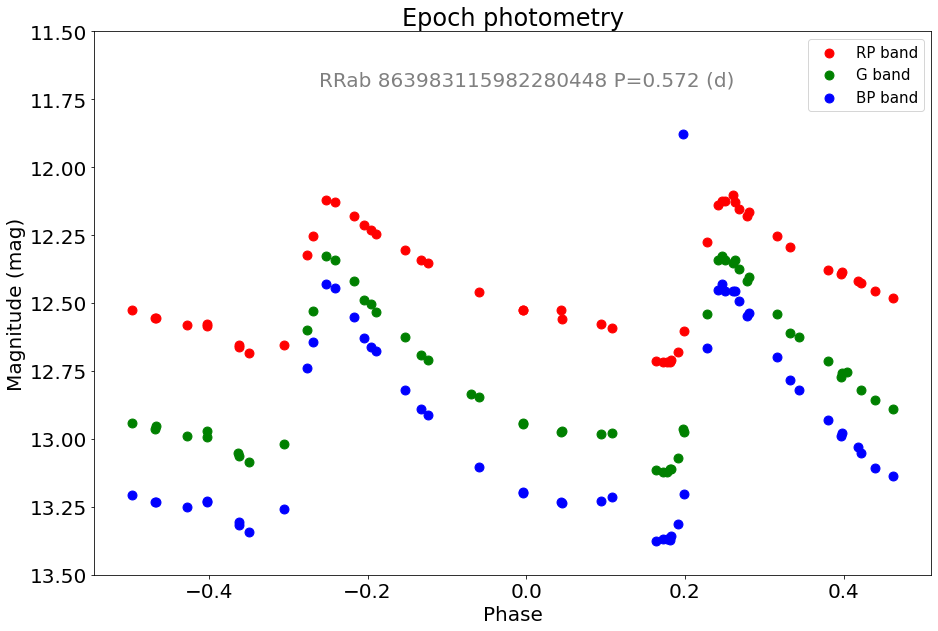
\includegraphics[scale=0.35]{lc_rrab_f.png}
\caption{Epoch photometry of the ab-type RR Lyrae Gaia DR3 863983115982280448 in the G, $G_{BP}$ and $G_{RP}$ bands in the phase domain. }
\label{fig:lightcurve_rrab_f}
\end{figure}



\begin{figure}[H]
\centering
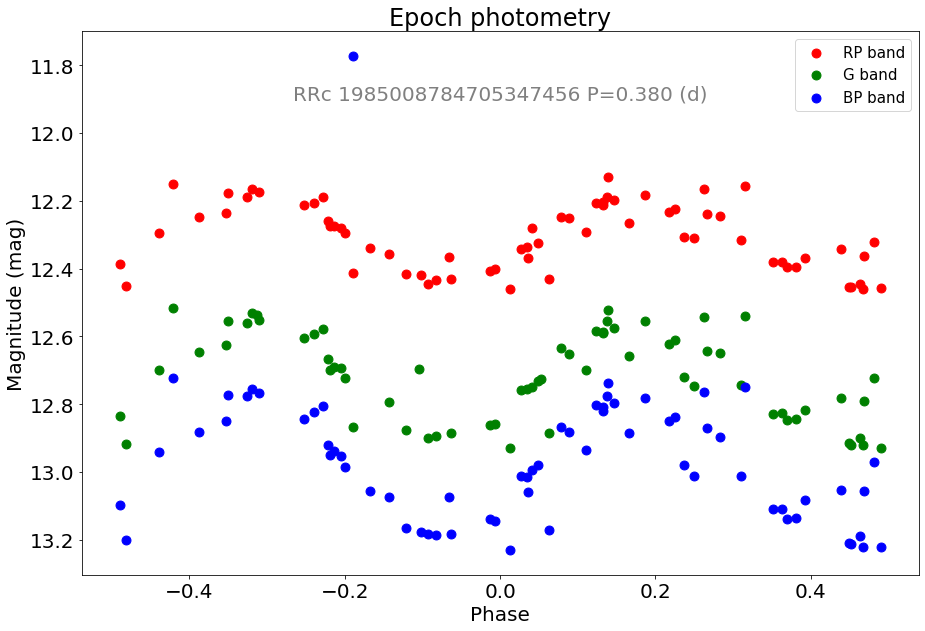
\includegraphics[scale=0.35]{lc_rrc_f.png}
\caption{Epoch photometry of the c-type RR Lyrae Gaia DR3 1985008784705347456 in the G, $G_{BP}$ and $G_{RP}$ bands in the phase domain. }
\label{fig:lightcurve_rrc_f}
\end{figure}


\begin{figure}[H]
\centering
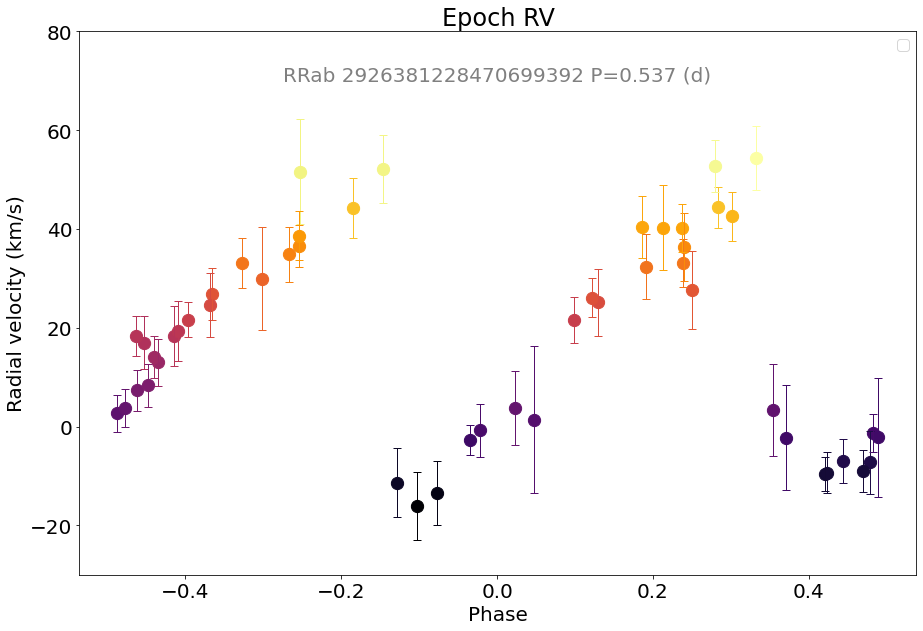
\includegraphics[scale=0.35]{rv_rrab.png}
\caption{Epoch radial velocity of the ab-type RR Lyrae Gaia DR3 2926381228470699392 in the phase domain. }
\label{fig:rv_rrab}
\end{figure}



\begin{figure}[H]
\centering
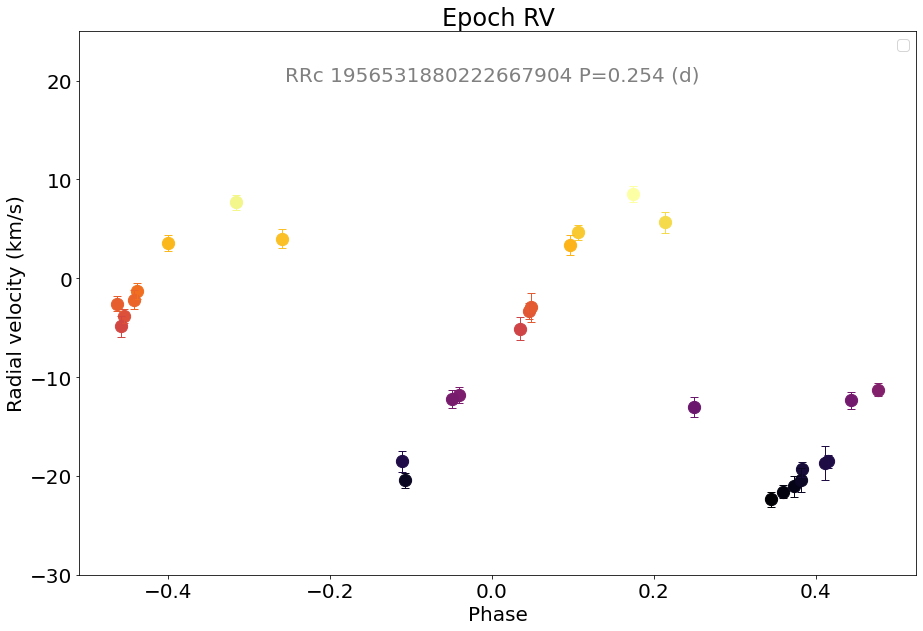
\includegraphics[scale=0.35]{rv_rrc.png}
\caption{Epoch radial velocity of the c-type RR Lyrae Gaia DR3 1956531880222667904 in the phase domain. }
\label{fig:rv_rrc}
\end{figure}


\newpage

\section{Solar-like variables}



For solar-like variable stars \parencite{refId8}, the flux variability is induced by the presence and the evolution of magnetically active regions (MARs), such as dark spots and bright faculae.
These magnetically active stars present a selection of variability phenomena whose time-scales can range between
few minutes, as in the case of flare events, to years, as in the
case of the periodic 11-yrs cycle observed in the Sun.\\
At an intermediate time-scale, solar-like
stars’ light curves display a rotational modulation signal, which is a quasi-periodic flux variation induced by the stellar rotation
that modulates the visibility of MARs over the stellar disk.

The galactic distribution of these variable sources as they are collected in the PLATO Input Catalogue is shown in fig. \ref{fig:All-sky map of solar-like variables}, while fig. \ref{fig:Absolute CMD} displays their absolute CMD corrected for extinction. 

The photometric amplitude A of the rotational modulation signal can be regarded as a proxy of the stellar magnetic activity level, which increases towards shorter rotation periods together with the MARs lifetime; moreover from the period of the rotational modulation signal the stellar rotation period can be inferred. 
The relationship between A and P can be observed in the density map reported in fig. \ref{fig:rot_pa.png}, which shows as expected from the literature the presence of three families of rotating stars, classified as Low-Amplitude-Slow-Rotators (LASR),  Low-Amplitude-Fast-Rotators (LAFR), and High-Amplitude-Rotators (HAR).\\
\begin{comment}
The data points could have been color-coded according to the Pearson Correlation Coefficient $r_0$(G, ($G_{BP}$ - $G_{RP}$)) measured in the whole time-series. From the plot it could have been inferred that HAR variables exhibit a strong positive correlation between magnitude and colour variations: as their brightness decreases their colour gets redder.
\end{comment}
The rotational modulation signal looses coherence and stability across the full Gaia photometric time-series because of the intrinsic evolution of MARs and can be detected only in shorter sub-series, whose duration is comparable with the spots life-time.
Therefore when analyzing epoch photometry it is necessary to perform a segmentation of the time-series, where each segment presents a significant period according to which the light curve can be folded.
This can be observed in fig. \ref{fig:rotation_modulation}, where the light curve of the solar-like star Gaia DR3 3934503103368181 is displayed.


\begin{comment}
The best estimate for the stellar rotation period (supplied as
best_rotation_period in the gdr3_rotmod catalog) is com-
puted by taking the mode of the significant periods distribution.
Each time-series segment, in which a significant period P
is detected, is folded according to P.

the Gaia scanning law favors the detection of stars with short rotation periods (P < 5 d).

# parameters 
-general colour–colour relation followed by most solar-like sources in the literature (with a model of G − G RP given G BP − G RP
-patterns of magnitude-colour variations for thousands of magnetically active stars
\end{comment}













\begin{figure}[H]
\centering
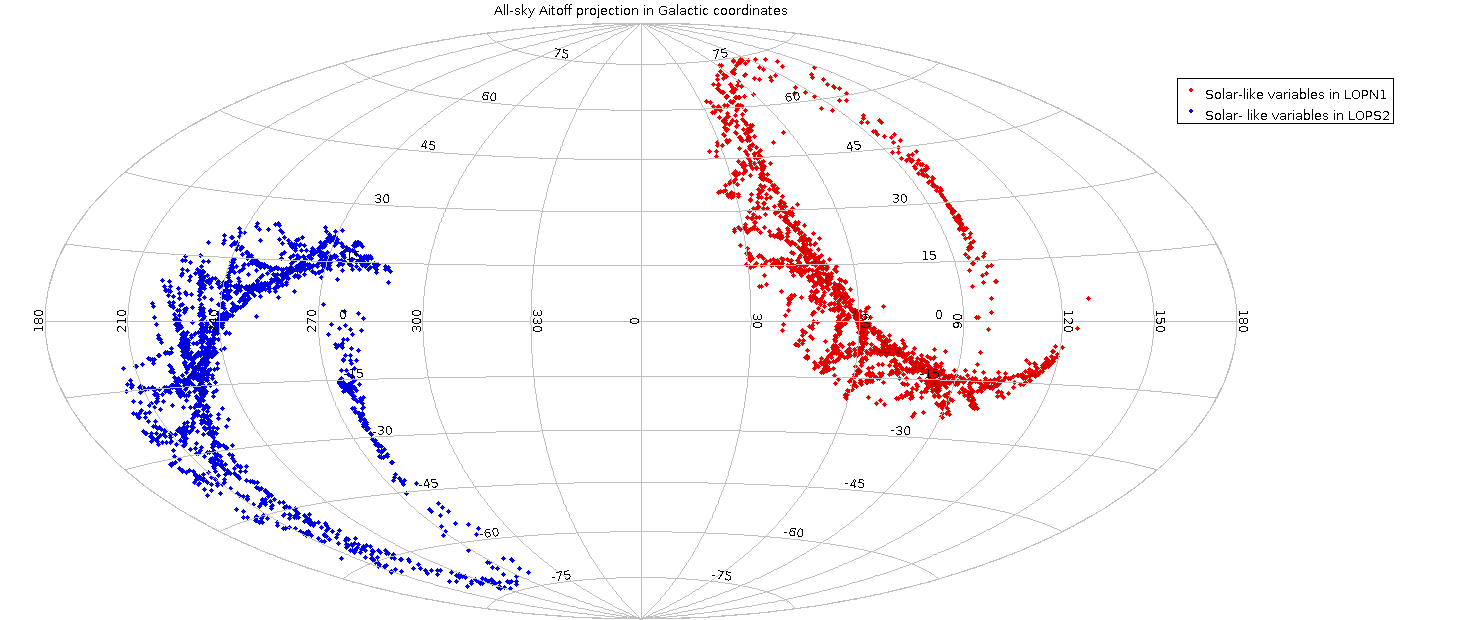
\includegraphics[scale=0.35]{rot_aitoff.png}
\caption{Sky map of solar-like variable stars in Galactic coordinates }
\label{fig:All-sky map of solar-like variables}
\end{figure}


\begin{comment}
\begin{figure}[H]
\centering
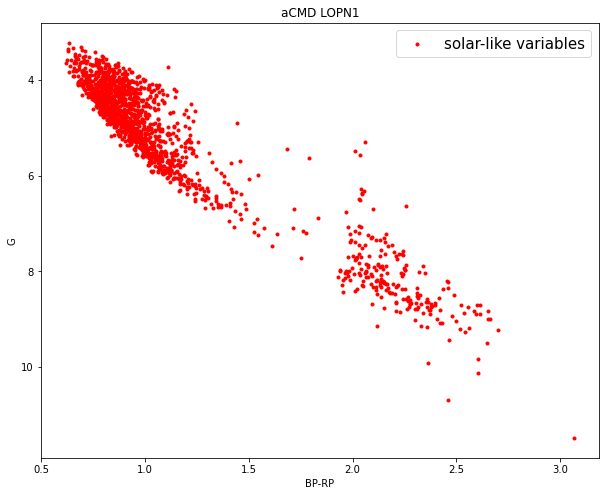
\includegraphics[scale=0.5]{rot_cmd.png}
\caption{Absolute CMD corrected for extinction for the solar-like variables in LOPN1}
\label{fig:Absolute CMD corrected for extinction for the solar-like variables in LOPN1}
\end{figure}


\begin{figure}[H]
\centering
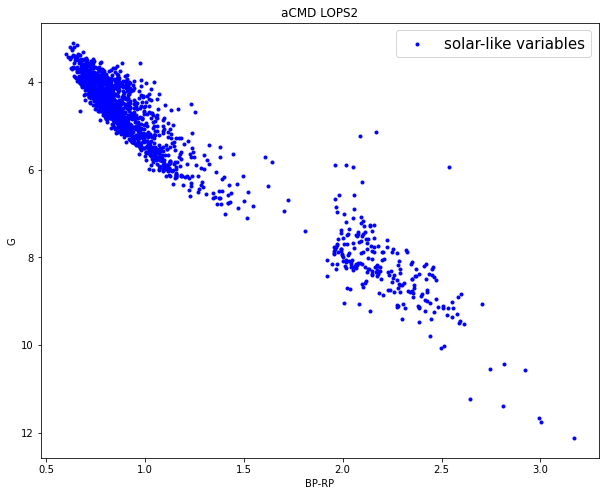
\includegraphics[scale=0.5]{rot2_cmd.png}
\caption{Absolute CMD corrected for extinction for the solar-like variables in LOPS2}
\label{fig:Absolute CMD corrected for extinction for the solar-like variables in LOPS2}
\end{figure}
\end{comment}

\begin{figure}[H]
\centering
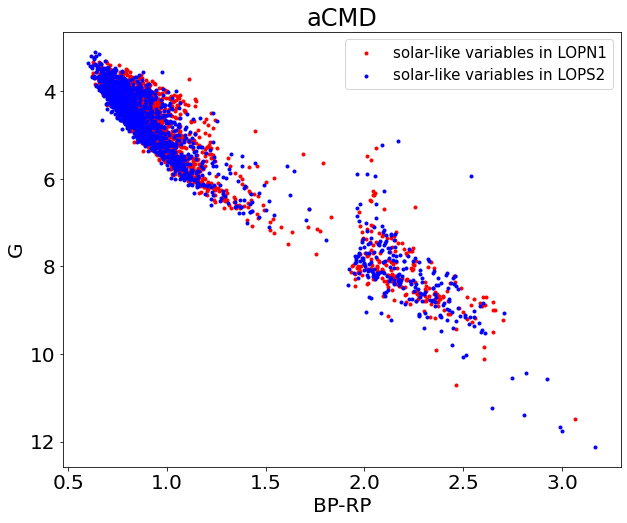
\includegraphics[scale=0.5]{rot_acmd.png}
\caption{Absolute CMD corrected for extinction for the total sample of solar-like variables in PIC}
\label{fig:Absolute CMD}
\end{figure}


\begin{figure}[H]
\centering
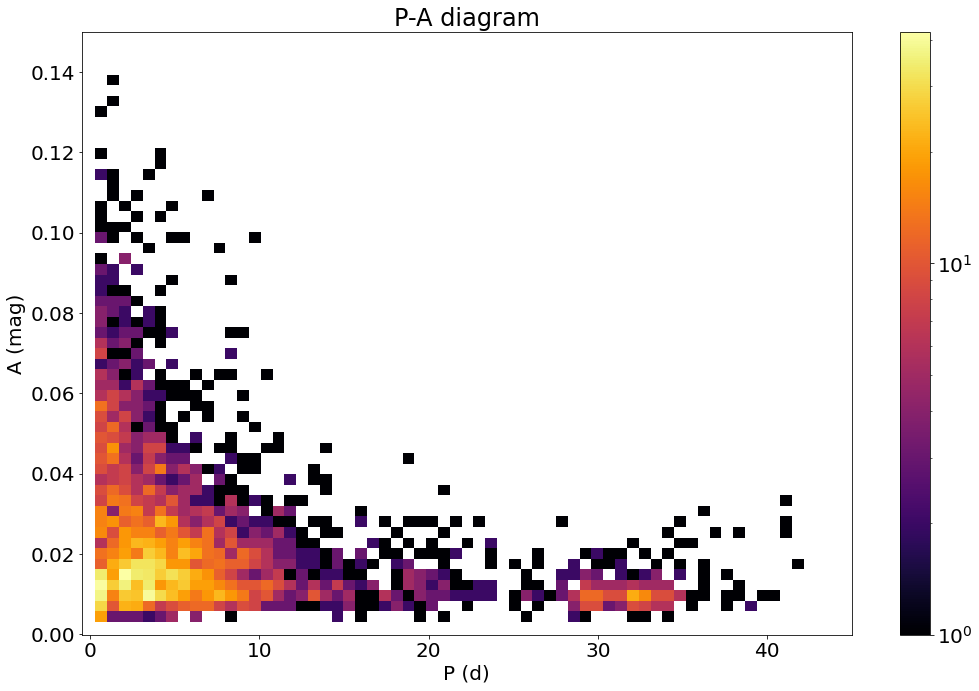
\includegraphics[scale=0.35]{rot_pa.png}
\caption{Period-Amplitude diagram for the total sample of solar-like variables in PIC}
\label{fig:rot_pa.png}
\end{figure}


\begin{figure}[H]
\centering
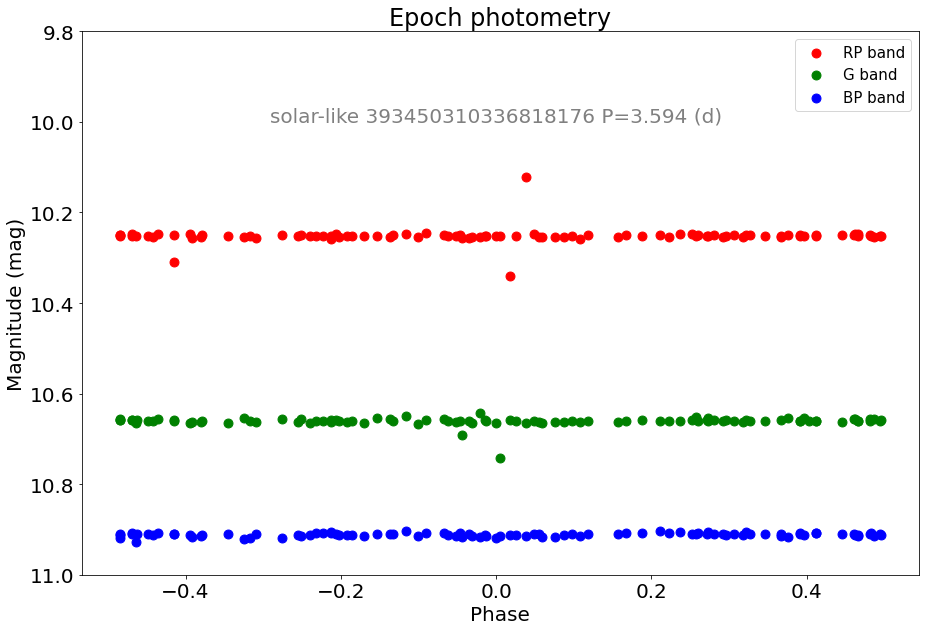
\includegraphics[scale=0.3]{phot1.png}
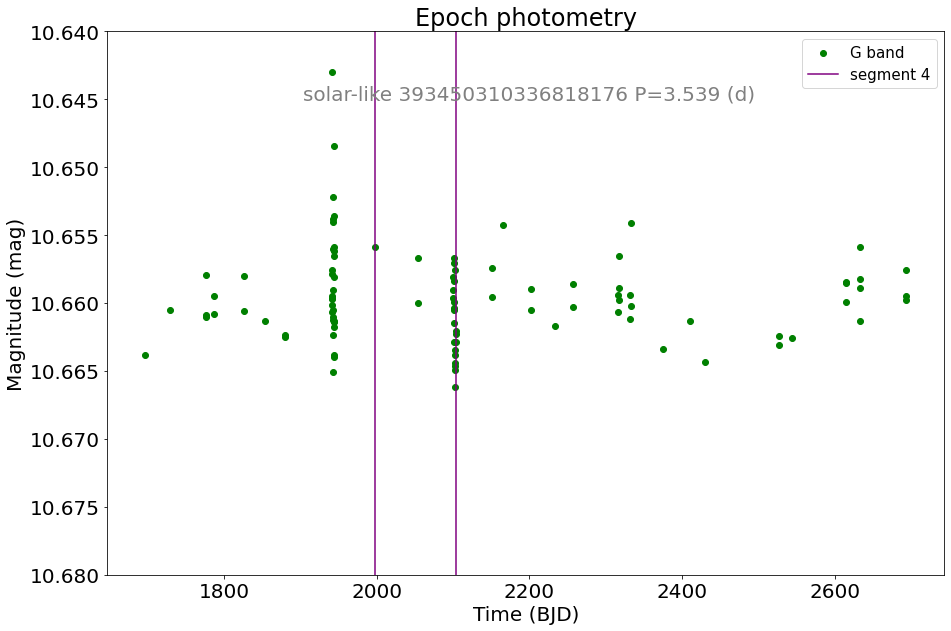
\includegraphics[scale=0.3]{phot2.png}
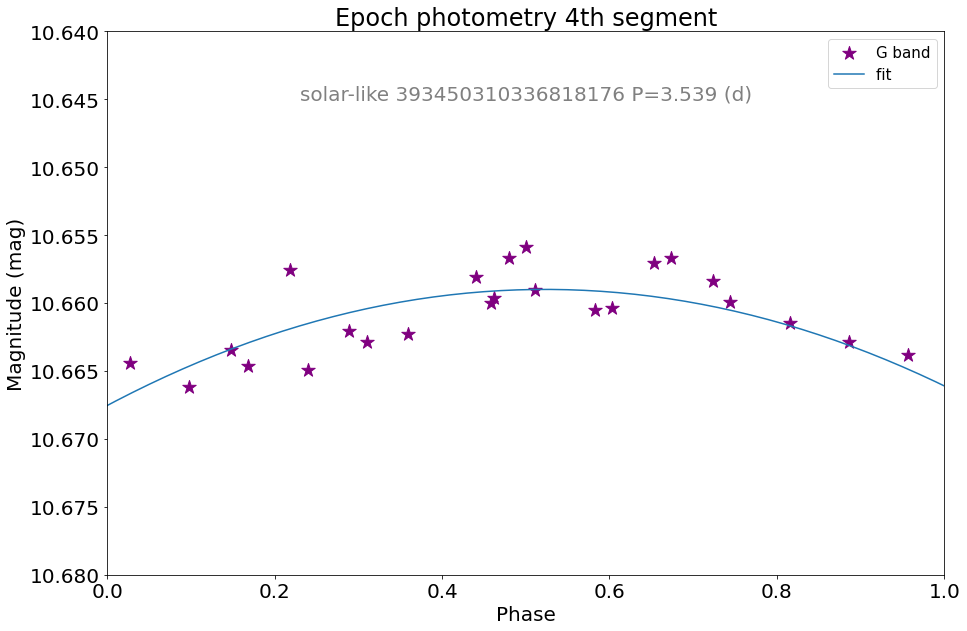
\includegraphics[scale=0.3]{phot3.png}
\caption{Top panel: full G, $G_{BP}$ and $G_{RP}$ time-series for the star Gaia DR3 393450310336818176 folded over the best rotation period P =  3.594 d.
Middle panel: full G time-series, where the purple vertical lines enclose the fourth segment.
Bottom panel: fourth sub-series folded according to the segment period P = 3.539 d and fitted by a sinusoidal curve.}
\label{fig:rotation_modulation}
\end{figure}





\newpage

\section{Main Sequence oscillators}

This sample of variable sources collected in the PLATO Input Catalogue include intermediate-to-high mass upper Main Sequence pulsators of spectral types early-F and hotter; among them SX Phoenicis, $\gamma$ Doradus and $\delta$ Scuti stars can be distinguished, the latter being the most populated variability class.\\
These non-radial oscillators are often multi-periodic, display very low amplitudes and typically a significant frequency peak  can be observed in the Fourier spectrum of their Gaia light curve, associated to a dominant oscillation mode \parencite{refId2}.\\
The sky map distribution of the considered sample of upper-MS oscillators is reported in figure \ref{fig:All-sky map of Main Sequence oscillators}; having convective cores, they occupy the so-called instability strips on the Hertzsprung-Russell (HR) diagram, shown in figure \ref{fig:ms_cmd}.\\
In fig. \ref{fig:af} and \ref{fig:histf} the distribution of the photometric amplitude in the G-band as a function of the primary frequency, and the histogram of the primary frequency can be observed respectively.\\
From the literature \parencite{refId2} $\delta$ Scuti stars are known to exhibit an empirical relation between their period and their luminosity: the period- Wesenheit G index diagram for our sample of stars is reported in figure \ref{fig:pw}, which shows two main clusters of pulsators presenting different oscillation regimes. 
The difference between fast rotating pulsators and slow-to-moderate pulsators arises from the physics of their internal rotation and core
convection.\\
Moreover, from the photometric G-band amplitude-projected rotational velocity plot displayed in fig. \ref{fig:av} it can be observed that stellar rotation attenuates the amplitude of the dominant oscillation mode of $\delta$ Sct stars, as expected: indeed even from the reduced available sample of stars provided with rotational velocity measurements, it appears that high amplitude sources tend to rotate slower, while the oscillation amplitude decreases for increasing rotational velocities.\\
The full time-series in the G, $G_{BP}$ and $G_{RP}$ bands for the star Gaia DR3 39332606552108761 and the phase diagram for the
same source folded according to its primary frequency are displayed in figure \ref{fig:ms}.






\begin{figure}[H]
\centering
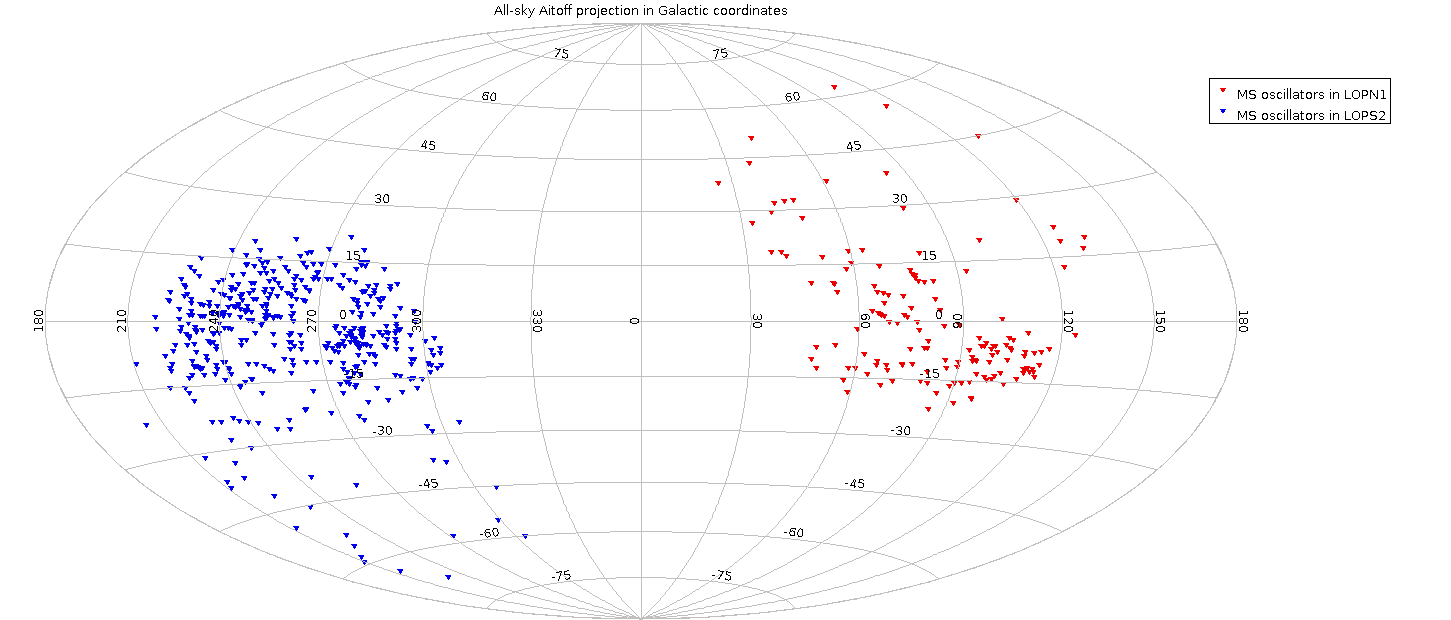
\includegraphics[scale=0.35]{MS_aitoff.png}
\caption{Sky map of Main Sequence oscillators in Galactic coordinates }
\label{fig:All-sky map of Main Sequence oscillators}
\end{figure}


\begin{comment}
\begin{figure}[H]
\centering
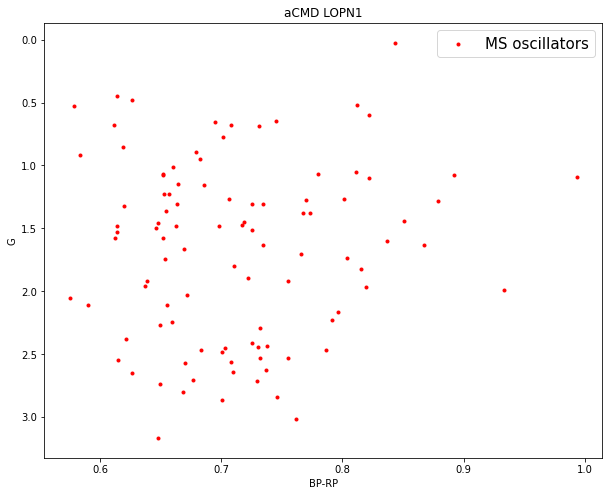
\includegraphics[scale=0.5]{ms_cmd.png}
\caption{Absolute CMD corrected for extinction for the MS oscillators in LOPN1}
\label{fig:Absolute CMD corrected for extinction for the MS oscillators in LOPN1}
\end{figure}


\begin{figure}[H]
\centering
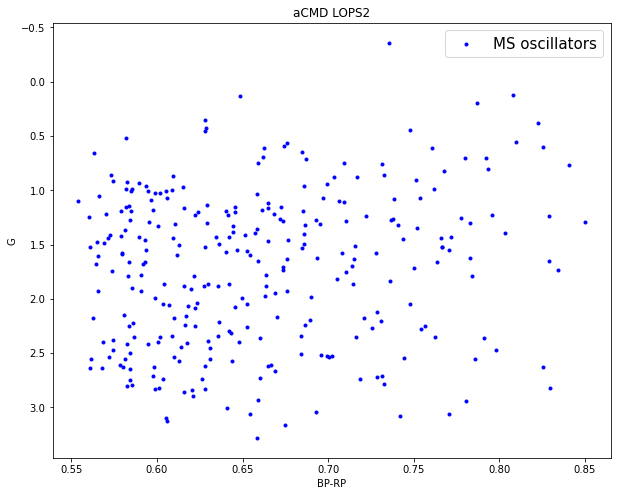
\includegraphics[scale=0.5]{ms2_cmd.png}
\caption{Absolute CMD corrected for extinction for the MS oscillators in LOPS2}
\label{fig:Absolute CMD corrected for extinction for the solar-like variables in LOPS2}
\end{figure}
\end{comment}

\begin{figure}[H]
\centering
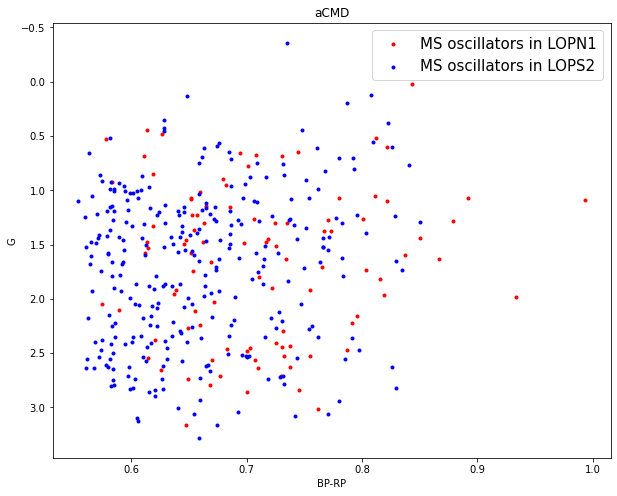
\includegraphics[scale=0.5]{ms_acmd.png}
\caption{Absolute CMD corrected for extinction for the total sample of MS oscillators in PIC}
\label{fig:ms_cmd}
\end{figure}


\begin{figure}[H]
\centering
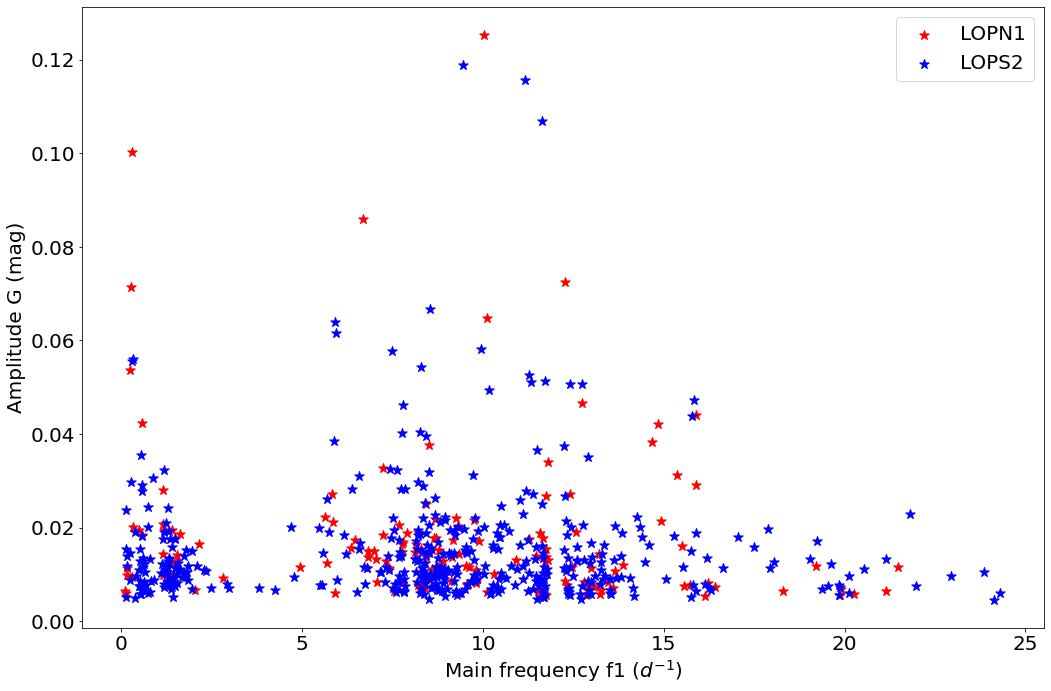
\includegraphics[scale=0.35]{af.png}
\caption{G-band amplitude-main frequency distribution}
\label{fig:af}
\end{figure}

\begin{figure}[H]
\centering
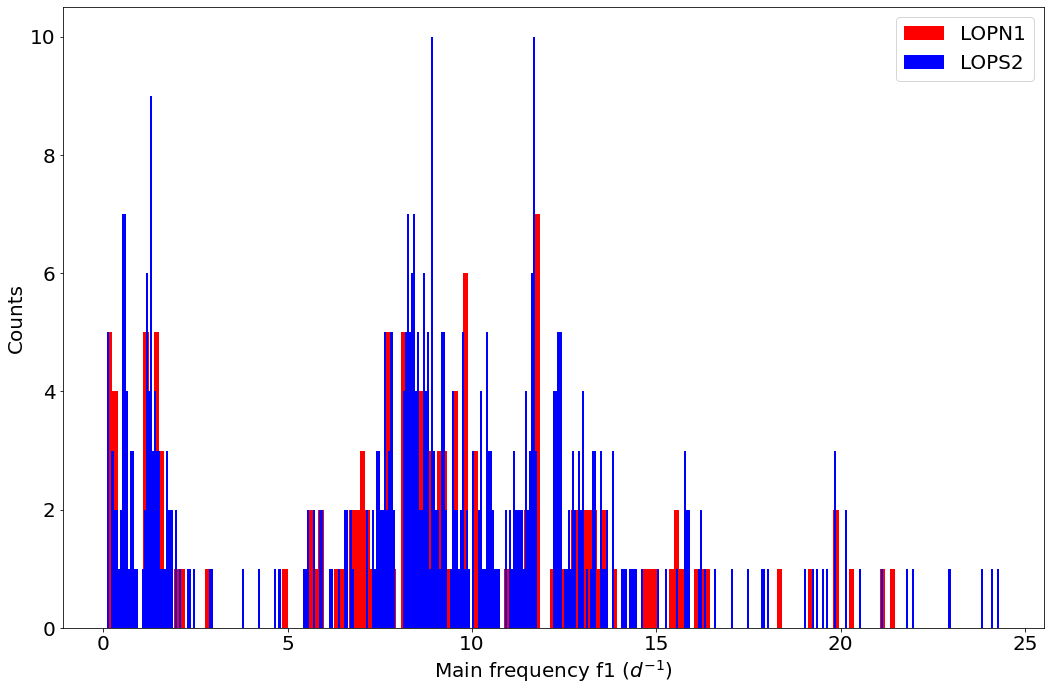
\includegraphics[scale=0.35]{histf.png}
\caption{Histogram of the primary frequency for the upper-MS pulsators of both LOP fields.}
\label{fig:histf}
\end{figure}


\begin{figure}[H]
\centering
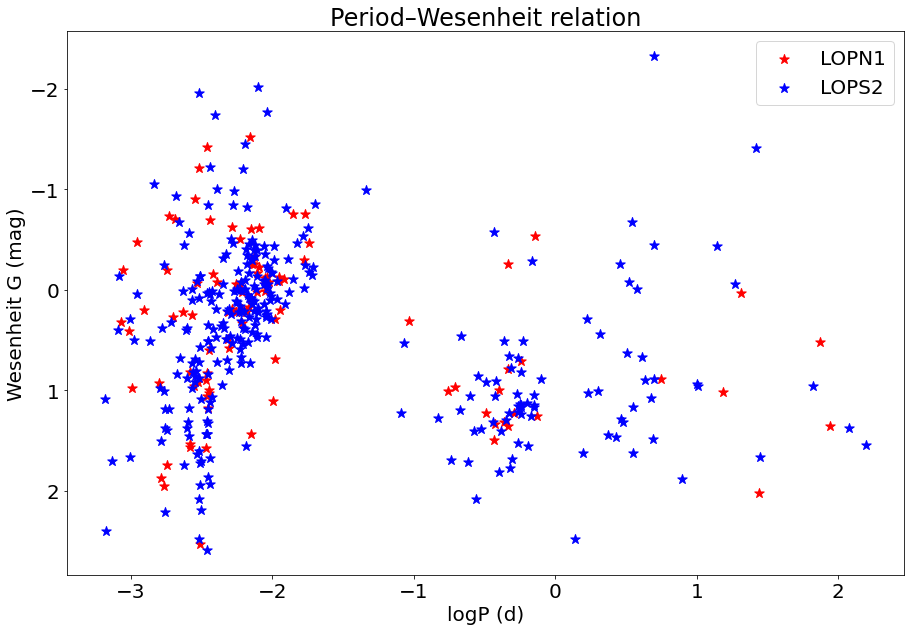
\includegraphics[scale=0.35]{pw.png}
\caption{Period-Wesenheit G diagram for the upper-MS pulsators of both LOP fields.}
\label{fig:pw}
\end{figure}

\begin{figure}[H]
\centering
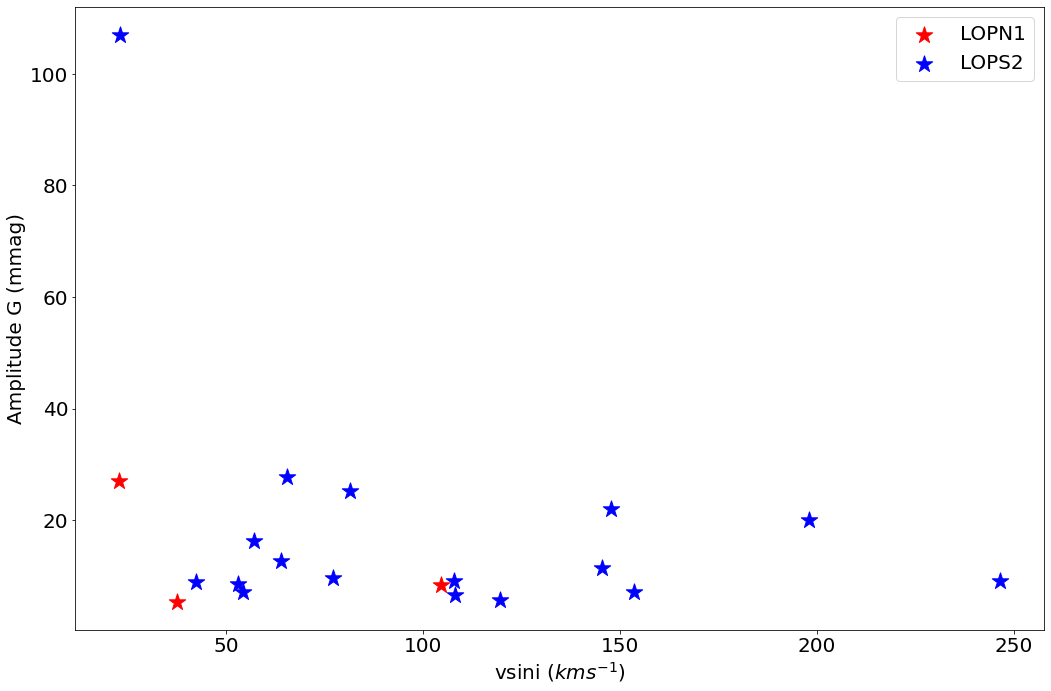
\includegraphics[scale=0.35]{av.png}
\caption{Photometric amplitude A in the Gaia G-band as a function
of the projected rotational velocity for a sample of $\delta$ Sct stars.}
\label{fig:av}
\end{figure}


\begin{figure}[H]
\centering
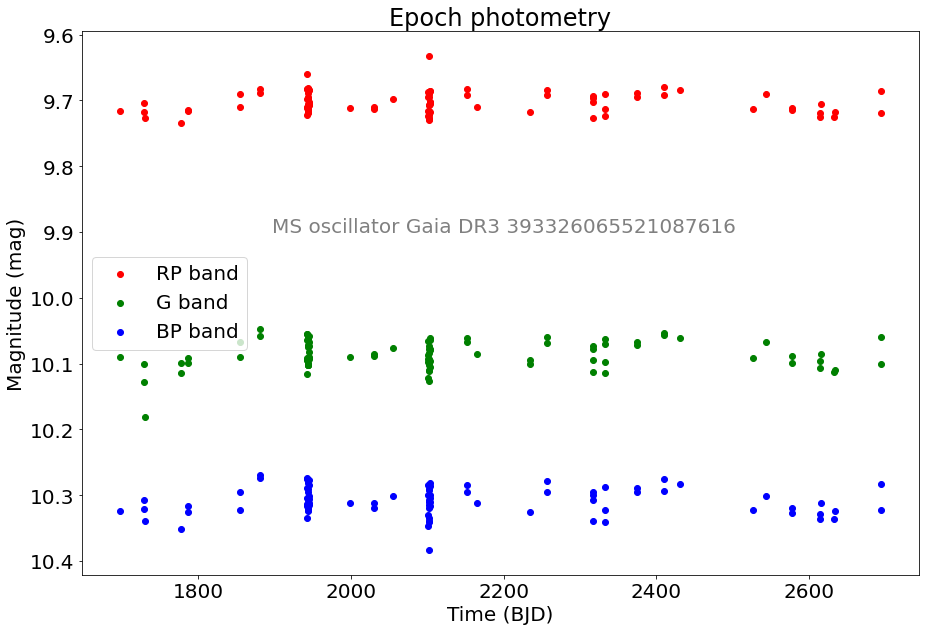
\includegraphics[scale=0.35]{ms_epoch.png}
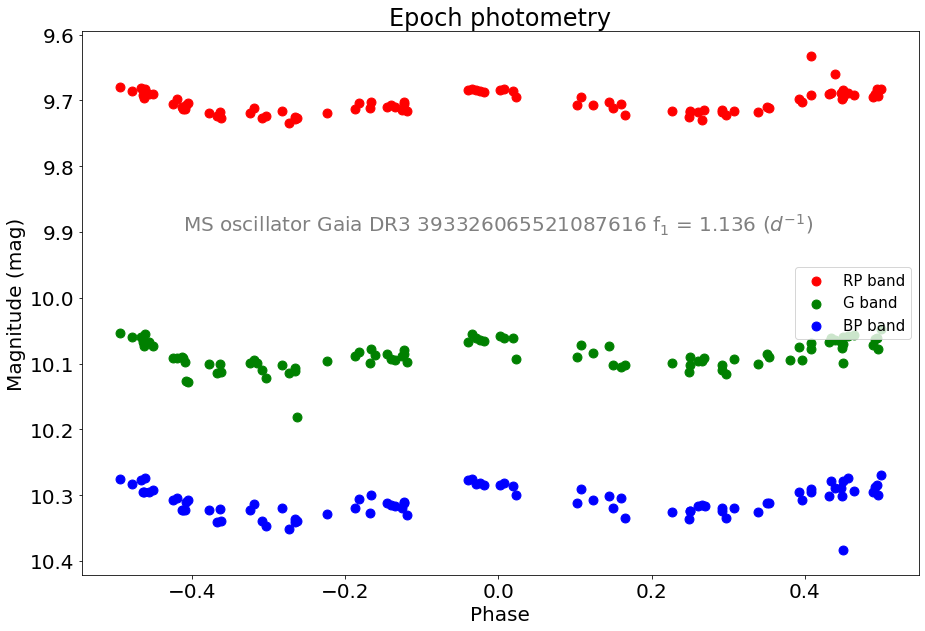
\includegraphics[scale=0.35]{ms_phase.png}
\caption{Top: photometric time series for the pre MS oscillator Gaia DR3 393326065521087616 in the G, $G_{BP}$ and $G_{RP}$ bands.
Bottom: phase diagram for the same source folded according to its primary frequency.}
\label{fig:ms}
\end{figure}





\newpage

\section{Planetary transits}



This class of photometric variables includes Main Sequence F-type stars displaying signatures of exoplanetary transits. 
Thanks to the high spatial resolution and its multi-epoch photometry, and despite its sparse and low-cadence observations, Gaia can identify false-positive candidates and confirm true detections of transiting planets from TESS exoplanetary candidates.
Indeed \cite{Panahi_2022} have confirmed the mission's very first two new Hot-Jupiters via RV follow up observations, Gaia-1b and Gaia-2b.

The Gaia DR3 planetary transits SOS module is composed of 173 known exoplanets with visible transits in the photometry of Gaia and 41 new candidates; the sample has been obtained through a a dedicated implementation of the BLS algorithm with the aim of searching for significant transit-like signals in the candidates light curves in the Full-Frame Image (FFI) photometry of TESS.

The known confirmed and the candidate transiting extra-solar planet hosts that are included in the PLATO Input Catalogue are collected in tables \ref{tab:planet1} and \ref{tab:planet2} respectively for the two Long-duration Observation Phase pointing fields.
Specifically 3 out of 21 are candidate exoplanetary hosts in the northern LOP field, while 7 out of 31 are the candidates in the southern LOP field.

The sky distribution of the PIC planetary transit events (whether alleged or confirmed) in Galactic coordinates and in Aitoff projection is shown in figure \ref{fig:All-sky map of extra-solar planets}; their observational Hertzsprung-Russell diagram is reported in figure \ref{fig:Absolute CMD corrected for extinction for the total sample of planet hosts in PIC}.



Figure \ref{fig:planetary} displays the lightcurve of the confirmed exoplanetary host KELT-16 (Gaia DR3 \textit{source\_id} 1864885215233116032), a yellow-white star of spectral class F7V closely orbited by a hot Jupiter; in figure \ref{fig:candidate} instead  the lightcurve of the candidate exoplanetary host TYC 3970-844-1 (Gaia DR3 \textit{source\_id} 2177849036734191744) is reported.



\begin{table}[H]
    
    \newcounter{mpFootnoteValueSaver}
    \begin{minipage}{\textwidth}
    \setcounter{mpFootnoteValueSaver}{\value{footnote}} \centering
   
    \begin{tabular}{c c c c c}
        \hline 
        \hline 
        Gaia DR3 \textit{source\_id} & Main ID & Spectral type & Exoplanet & References \\
        \hline 
        1334573817793362560 & HAT-P-18 & K2V & HAT-P-18 b & \footnotemark{} \footnotemark{} \footnotemark{} \footnotemark{} \footnotemark{} \\
        1928431764627661440 & BD+37 4734B & G0V & HAT-P-1 b &  \footnotemark[1] \footnotemark[2] \footnotemark[3] \footnotemark[4] \footnotemark[5] \\
        1962153854973972096 & HAT-P-40 & F & HAT-P-40 b & \footnotemark[1] \footnotemark[2] \footnotemark[3] \footnotemark[4] \footnotemark[5] \\
        1316708918505350528  & BD+28 2507  & G1V  & XO-1 b & \footnotemark[1] \footnotemark[2] \footnotemark[3] \footnotemark[4] \footnotemark[5] \\
        1622997463177004928 & WISEA J160752.17+574902.9  &   & N/A  & \footnotemark[1] \footnotemark[4] \footnotemark{} \\
        1864885215233116032 & KELT-16 & F7V & KELT-16 b & \footnotemark[1] \footnotemark[2] \footnotemark[3] \footnotemark[4] \footnotemark[5] \\
        2262322556576778752 & Qatar-10  & F7V & Qatar-10 b  & \footnotemark[1] \footnotemark[2] \footnotemark[3] \footnotemark[4] \footnotemark[5]   \\
        2244830490514284928 & Qatar-1  & K  &  Qatar-1 b  & \footnotemark[1] \footnotemark[2] \footnotemark[3] \footnotemark[4] \footnotemark[5]  \\
        1424011082893734272 & WASP-92  & F7  & WASP-92 b  & \footnotemark[1] \footnotemark[2] \footnotemark[3] \footnotemark[4] \footnotemark[5]   \\
         4606030169272920320 & HAT-P-5  & G1V  & HAT-P-5 b  & \footnotemark[1] \footnotemark[2] \footnotemark[3] \footnotemark[4] \footnotemark[5]  \\
        2177849036734191744  & TYC 3970-844-1 &  & N/A & \footnotemark[1] \footnotemark[2] \footnotemark[4] \footnotemark[5] \\
       4609062308806929152  & TYC 2620-648-1  & F8  & TrES-4 b  & \footnotemark[1] \footnotemark[2] \footnotemark[3] \footnotemark[4] \footnotemark[5] \\
      4609131509318715136  & 1SWASP J175207.01+373246.3 & G & TrES-3 b &  \footnotemark[1] \footnotemark[2] \footnotemark[3] \footnotemark[4] \footnotemark[5] \\
      2102117871259036672  & Kepler-7  & G0  &  Kepler-7 b & \footnotemark[1] \footnotemark[2] \footnotemark[3] \footnotemark[4] \footnotemark[5] \\
      2129256395211984000  & BD+47 2846  & F6V  & HAT-P-7 b  & \footnotemark[1] \footnotemark[2] \footnotemark[3] \footnotemark[4] \footnotemark[5]  \\
      2141754578242371584  & WASP-48  & G0IV  & WASP-48 b  & \footnotemark[1] \footnotemark[2] \footnotemark[3] \footnotemark[4] \footnotemark[5]  \\
      1499514786891168640  & HAT-P-12  & K5 & HAT-P-12 b  & \footnotemark[1] \footnotemark[2] \footnotemark[3] \footnotemark[4] \footnotemark[5] \\
     4535127268607000320   & WISEA J183411.49+220908.4  &   & N/A  & \footnotemark[1] \footnotemark[4]  \footnotemark[6]  \\
      1644692064543192704  & BD+66 911  & K  & KELT-23A b  & \footnotemark[1] \footnotemark[2] \footnotemark[3] \footnotemark[4] \footnotemark[5]  \\
      1827242816201846144  & HD 189733  &  K2V & HD 189733 b  & \footnotemark[1] \footnotemark[2] \footnotemark[3] \footnotemark[4] \footnotemark[5]   \\
     1587399232335653760   &  WASP-113 & G1  & WASP-113 b  & \footnotemark[1] \footnotemark[2] \footnotemark[3] \footnotemark[4] \footnotemark[5]  \\
         \hline 
    \end{tabular}
    \caption{List of the 21 confirmed and candidate transiting exoplanet hosts in LOPN1.\\}
    \label{tab:planet1}
    \end{minipage}
   \end{table}
  \vspace{8mm}

    
   \begin{table}
     \begin{tabular}{c c c c c}
        \hline 
        \hline 
        Gaia DR3 \textit{source\_id} & Main ID & Spectral type & Exoplanet & References \\
        \hline
        5345417757181174144 & WISEA J114230.50-523738.6  &   & N/A  & \footnotemark[1] \footnotemark[4] \footnotemark[6]  \\
        5608644895310998272 & HATS-51 & G & HATS-51 b & \footnotemark[1] \footnotemark[2] \footnotemark[3] \footnotemark[4] \footnotemark[5]   \\
       5594445630358459648  & 2MASS J07545687-3221219  &   &  N/A &   \footnotemark[1] \footnotemark[4] \footnotemark[6]  \\
       4895643593611507584  & WISEA J041929.55-255735.4  &   & N/A  & \footnotemark[1] \footnotemark[4] \footnotemark[6]  \\
       4899428146994060800  & HATS-5  & K0  & HATS-5 b  &  \footnotemark[1] \footnotemark[2] \footnotemark[3] \footnotemark[4] \footnotemark[5]  \\
        4906145613282734208 & HATS-30  & G1 & HATS-30 b  &  \footnotemark[1] \footnotemark[2] \footnotemark[3] \footnotemark[4] \footnotemark[5] \\
        4677436783705094912 &  WISEA J043143.94-612309.1 &   & N/A  &  \footnotemark[1] \footnotemark[4] \footnotemark[6]   \\
        5565050255701441664 &  CD-38 3220 &  F6V & WASP-121 b & \footnotemark[1] \footnotemark[2] \footnotemark[3] \footnotemark[4] \footnotemark[5]  \\
        5583523425437258240 & WASP-64  & G7  & WASP-64 b  & \footnotemark[1] \footnotemark[2] \footnotemark[3] \footnotemark[4] \footnotemark[5]  \\
        5578530470116727936  &  WISEA J070548.04-351521.8 &   & N/A  & \footnotemark[1] \footnotemark[4] \footnotemark[6]   \\
       3211188618762023424 & BD-06 1077  & G0  &  WASP-35 b  & \footnotemark[1] \footnotemark[2] \footnotemark[3] \footnotemark[4] \footnotemark[5]  \\
        5348534425968598400 &  TYC 8225-452-1 &   & N/A  &  \footnotemark[1] \footnotemark[2] \footnotemark[4] \footnotemark[5] \\
        4851398799032507776 & WASP-139  & K0  & WASP-139 b  &  \footnotemark[1] \footnotemark[2] \footnotemark[3] \footnotemark[4] \footnotemark[5] \\
        4864759888238232320 & WASP-159  & F9  &  WASP-159 b & \footnotemark[1] \footnotemark[2] \footnotemark[3] \footnotemark[4] \footnotemark[5]  \\
        4955371367334610048 &  HD 10069 & F6V  &  WASP-18 b &  \footnotemark[1] \footnotemark[2] \footnotemark[3] \footnotemark[4] \footnotemark[5]  \\
         2959177048983750016 & WASP-61  & F7  & WASP-61 b  & \footnotemark[1] \footnotemark[2] \footnotemark[3] \footnotemark[4] \footnotemark[5]  \\
         5656896924435896832 & HATS-26  & F  & HATS-26 b  & \footnotemark[1] \footnotemark[2] \footnotemark[3] \footnotemark[4] \footnotemark[5]  \\
        5444147952811517696  & WASP-66  & F4  & WASP-66 b  & \footnotemark[1] \footnotemark[2] \footnotemark[3] \footnotemark[4] \footnotemark[5]   \\
         5557345496687437696  & WASP-23  & K1V  & WASP-23 b  & \footnotemark[1] \footnotemark[2] \footnotemark[3] \footnotemark[4] \footnotemark[5]   \\
         4746157737910069888 & CD-50 714  & F9  & WASP-117 b  & \footnotemark[1] \footnotemark[2] \footnotemark[3] \footnotemark[4] \footnotemark[5]   \\
         5086537022856406272 & WASP-22  &  G &  WASP-22 b &  \footnotemark[1] \footnotemark[2] \footnotemark[3] \footnotemark[4] \footnotemark[5]  \\
         5089851638095503616 & WASP-78  & F8  & WASP-78 b  & \footnotemark[1] \footnotemark[2] \footnotemark[3] \footnotemark[4] \footnotemark[5]   \\
          6386751579018596864 & WASP-91  & K3  & WASP-91 b  & \footnotemark[1] \footnotemark[2] \footnotemark[3] \footnotemark[4] \footnotemark[5]   \\
         5735158757648658048 & UCAC4 384-050987  &   & N/A &  \footnotemark[1] \footnotemark[2] \footnotemark[4] \footnotemark[5] \\
         5262709709389254528 & TOI-150  &  F &  TOI-150 b & \footnotemark[1] \footnotemark[2] \footnotemark[3] \footnotemark[4] \footnotemark[5]   \\
         5560886336446650240 & CD-42 3043  & G4  & WASP-122 b  & \footnotemark[1] \footnotemark[2] \footnotemark[3] \footnotemark[4] \footnotemark[5]   \\
         2980392087185289216 & WASP-141  & F9  & WASP-141 b  & \footnotemark[1] \footnotemark[2] \footnotemark[3] \footnotemark[4] \footnotemark[5]  \\
         5489780919480009472 & CD-51 2720  & G0 & KELT-15 b  & \footnotemark[1] \footnotemark[2] \footnotemark[3] \footnotemark[4] \footnotemark[5]   \\
         4911563216311083392 & CD-56 324  & G5  & WASP-97 b  &  \footnotemark[1] \footnotemark[2] \footnotemark[3] \footnotemark[4] \footnotemark[5]  \\
         2991284369063612928 & WASP-49  & G6V  &  WASP-49 A b & \footnotemark[1] \footnotemark[2] \footnotemark[3] \footnotemark[4] \footnotemark[5]   \\
         5723772524469252096 &  WASP-169 & G0  & WASP-169 b  & \footnotemark[1] \footnotemark[2] \footnotemark[3] \footnotemark[4] \footnotemark[5]   \\
         \hline 
    \end{tabular}  
    \caption{List of the 31 confirmed and candidate transiting exoplanet hosts in LOPS2.\\}
    \label{tab:planet2}

\end{table}


 \stepcounter{mpFootnoteValueSaver}
 \footnotetext[\value{mpFootnoteValueSaver}]{http://cdsportal.u-strasbg.fr/}
 \stepcounter{mpFootnoteValueSaver}
 \footnotetext[\value{mpFootnoteValueSaver}]{http://simbad.u-strasbg.fr/}
 \stepcounter{mpFootnoteValueSaver}
 \footnotetext[\value{mpFootnoteValueSaver}]{http://exoplanet.eu/catalog/}
 \stepcounter{mpFootnoteValueSaver}
 \footnotetext[\value{mpFootnoteValueSaver}]{https://vizier.cds.unistra.fr/}
 \stepcounter{mpFootnoteValueSaver}
 \footnotetext[\value{mpFootnoteValueSaver}]{https://exofop.ipac.caltech.edu/tess/}
 \stepcounter{mpFootnoteValueSaver}
\footnotetext[\value{mpFootnoteValueSaver}]{https://ned.ipac.caltech.edu/}

%\footnotetext{https://exofop.ipac.caltech.edu/tess/}


% Gaia DR3 16075215+5749031: RSG SRc type stars are semiregular late-type supergiants with amplitudes of about 1 mag and periods from 30 d to several thousand days.





\begin{figure}[H]
\centering
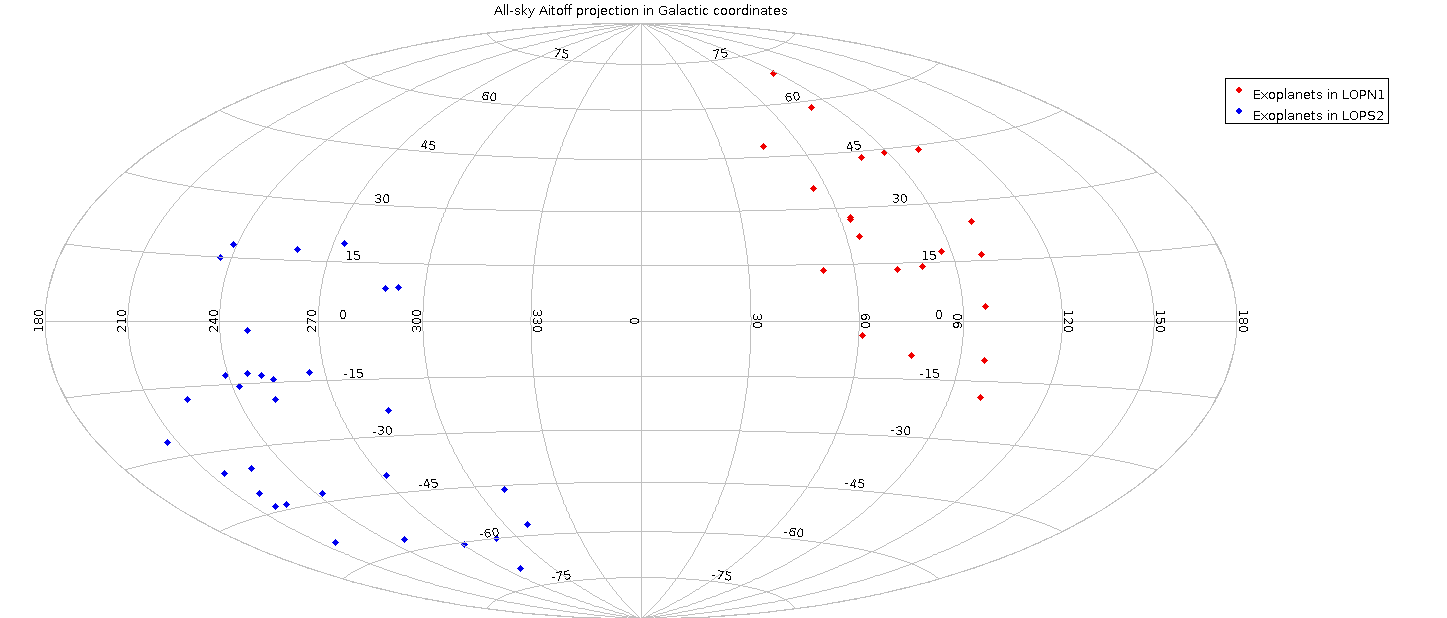
\includegraphics[scale=0.35]{EP_aitoff.png}
\caption{Sky map of variable stars showing planetary transits signals in Galactic coordinates }
\label{fig:All-sky map of extra-solar planets}
\end{figure}

\begin{comment}
\begin{figure}[H]
\centering
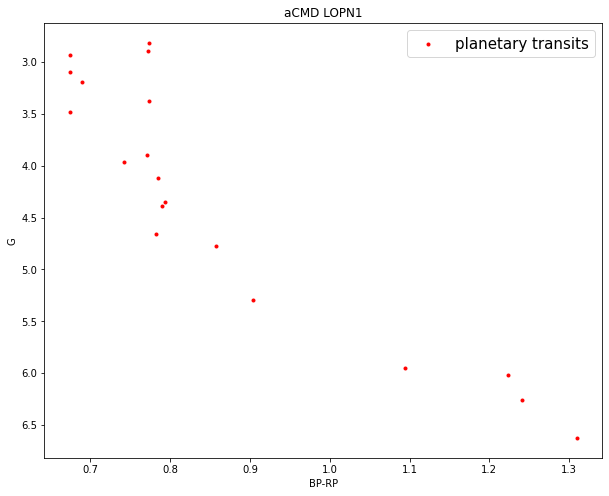
\includegraphics[scale=0.5]{ep_cmd.png}
\caption{Absolute CMD corrected for extinction for the planet hosts in LOPN1}
\label{fig:Absolute CMD corrected for extinction for the planet hosts in LOPN1}
\end{figure}


\begin{figure}[H]
\centering
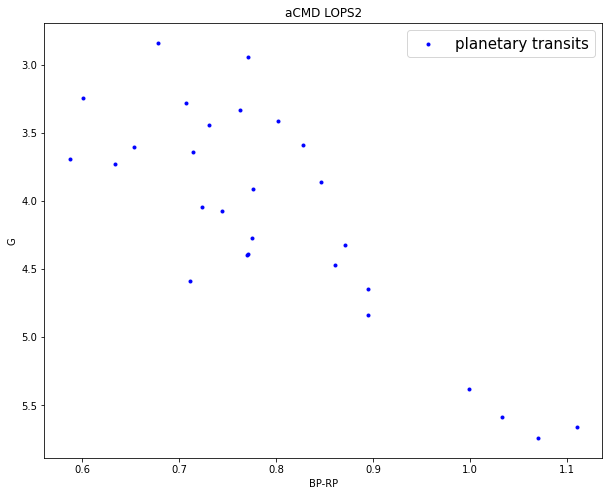
\includegraphics[scale=0.5]{ep2_cmd.png}
\caption{Absolute CMD corrected for extinction for the planet hosts in LOPS2}
\label{fig:Absolute CMD corrected for extinction for the planet hosts in LOPS2}
\end{figure}
\end{comment}

\begin{figure}[H]
\centering
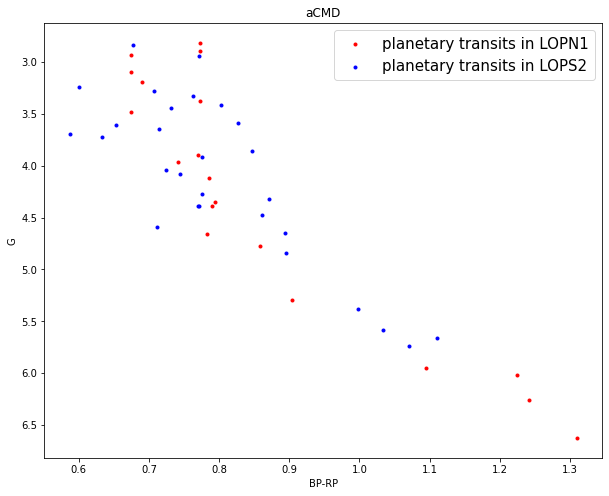
\includegraphics[scale=0.5]{ep_acmd.png}
\caption{Absolute CMD corrected for extinction for the total sample of planet hosts in PIC}
\label{fig:Absolute CMD corrected for extinction for the total sample of planet hosts in PIC}
\end{figure}


\begin{figure}[H]
\centering
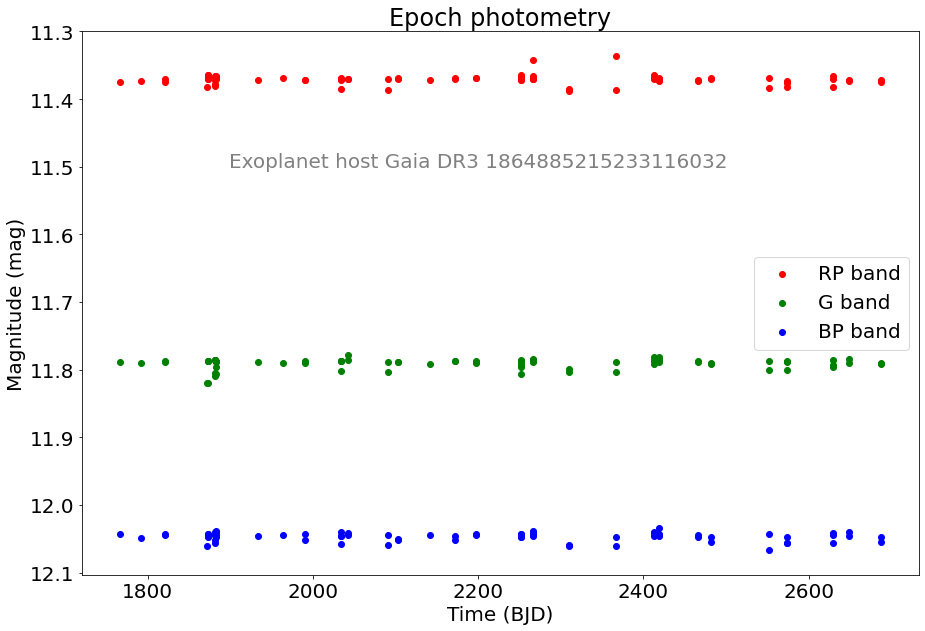
\includegraphics[scale=0.3]{planet1.png}
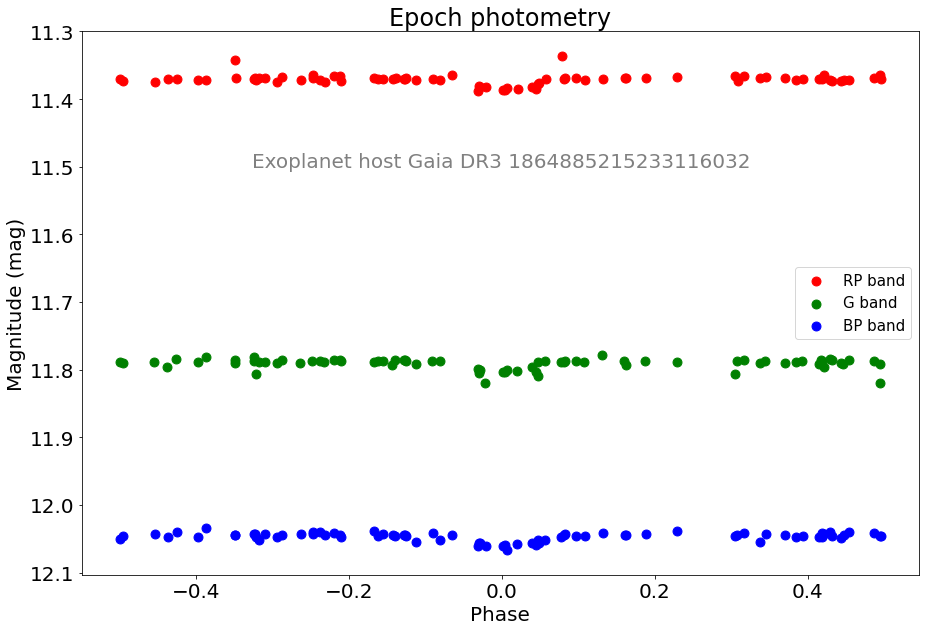
\includegraphics[scale=0.3]{planet2.png}
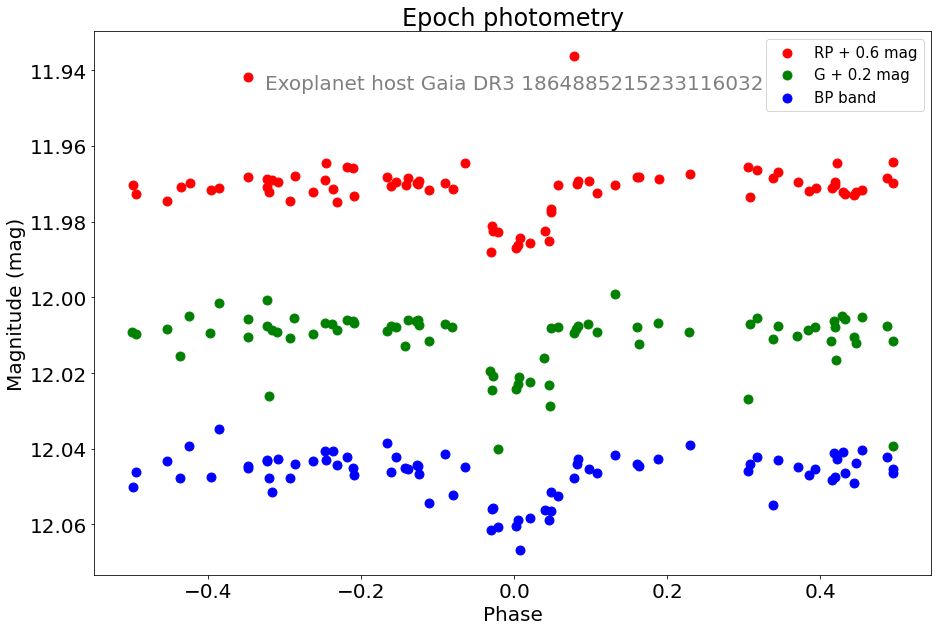
\includegraphics[scale=0.3]{planet3.png}
\caption{Top panel: full time-series in the G, $G_{BP}$ and $G_{RP}$ bands for the extra-solar planet host KELT-16 (Gaia DR3 1864885215233116032).
Middle panel: phase-folded light curves according to the transit orbital period P = 0.97 d.
Bottom panel: zoom on the phase diagram displaying the transit event in the three photometric bands. }
\label{fig:planetary}
\end{figure}


\begin{figure}[H]
\centering
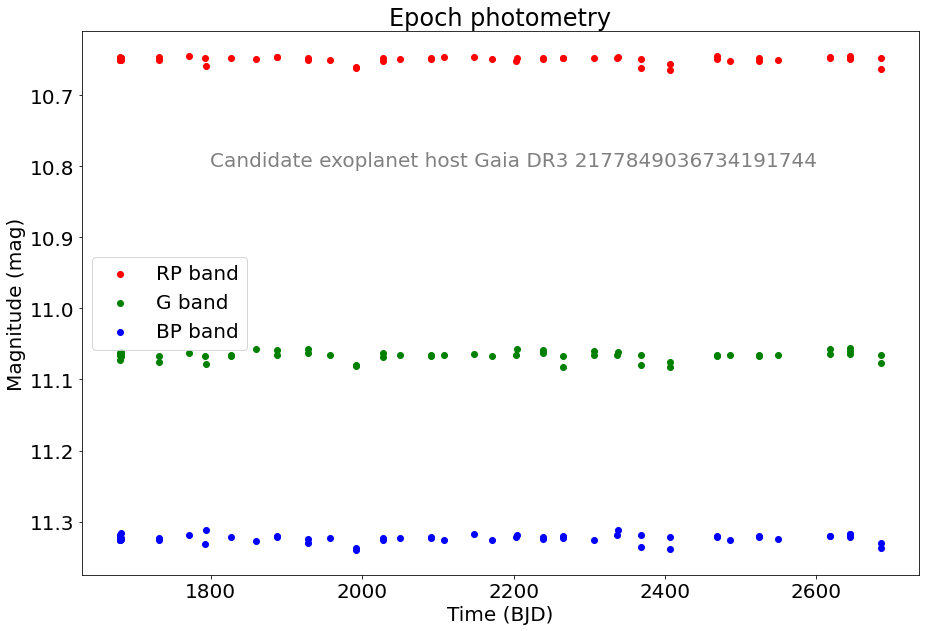
\includegraphics[scale=0.3]{candid1.png}
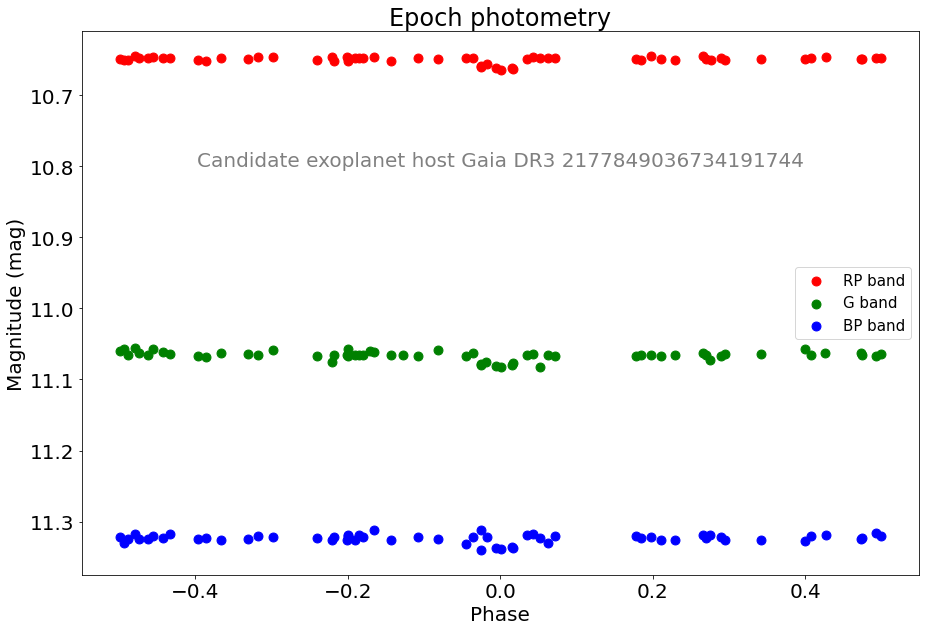
\includegraphics[scale=0.3]{candid2.png}
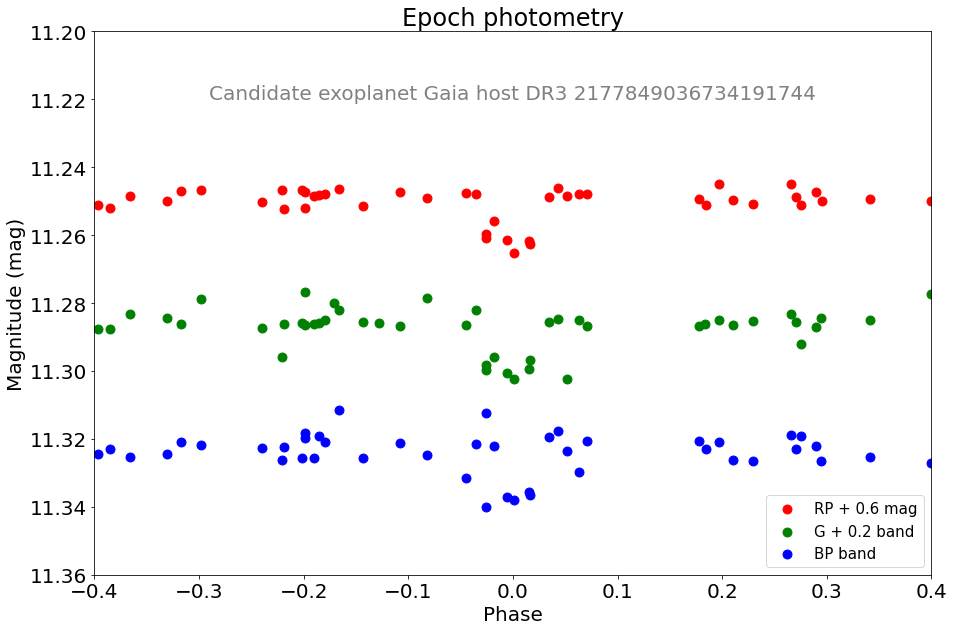
\includegraphics[scale=0.3]{candid3.png}
\caption{Same as figure 3.24 but for the candidate exoplanetary host Gaia DR3 2177849036734191744 (TYC 3970-844-1).
The light curves in the middle and bottom panels have been folded according to the period P = 3.81 d. }
\label{fig:candidate}
\end{figure}








\newpage

\section{Eclipsing binaries}

While the majority of stars is in binary systems, only a fraction of them appears to the observer as eclipsing; this family is of capital importance, since eclipsing binaries allow to derive the stars' physical and orbital parameters, play a fundamental role in stellar evolution and their eccentricity can be used as a test for the theory of general relativity.
Moreover from variations in the eclipse timings the presence of extra-solar planets can be inferred.\\
Gaia DR3 Catalogue contains 813687 unique non-single star sources between astrometric, spectroscopic, photometric binaries and higher order stellar systems \parencite{arenou}; moreover it includes the largest collection to date (2184477 sources) of eclipsing binaries (86918 of which provided with orbital solutions), whose brightnesses span from a few magnitudes to 20 mag in the Gaia G-band \parencite{mowlavi2022gaia}.\\
% an Algol-type eclipsing binary, is one in which a star that fills its Roche lobe is much fainter than its companion
% EW-type eclipsing binaries vary on short timescales.
The PLATO Input Catalogue features Algol ($\beta$ Persei) type (EA), $\beta$ Lyrae type (EB), and W Ursae Majoris type (EW) eclipsing binaries, distributed between the northern (2977 sources) and southern (3466 sources) observation fields.

Their distributions in the Aitoff Galactic projection and in the observational Hertzsprung–Russell diagram are shown in figures \ref{fig:All-sky map of eclipsing binaries} and \ref{fig:Absolute CMD corrected for extinction for the total sample of eclipsing binaries in PIC} respectively.

It is possible to identify different groups of eclipsing binaries among the sample, from wide (P $>$ 50 d) to tight (P $<$ 10 d) systems, in the orbital period histogram displayed in figure \ref{fig:periodhisto_eb}.

The G, $G_{RP}$ and $G_{BP}$ light curves of the eclipsing binary Gaia DR3 393454948901343360 is shown in figure \ref{fig:binary}, where the gaussian shape of the primary eclipse is clearly visible at phase = 0.2.

%The geometry of the G-band light curves is modelled with a combination of Gaussian functions to approximate the eclipses and a sine function to model any ellipsoidal variability due to deformation of one or both components in the binary

%The ratio between G BP and G RP amplitudes is close to one (Fig. E.26g), as expected from non-pulsating objects (apart from the increasing scatter towards faint magnitudes due to shot noise). Low-amplitude and low-skewness candidates tend to be associated with low classification scores (Fig. E.26e,f).

%This catalogue of eclipsing binaries is purely based on the brightness variability and is complementary to the detailed non-single source analysis published in the different DR3 tables, e.g., nss two body orbit.
%Indeed in this table (under Non-single stars in the Gaia archive, with nss solution type=EclipsingBinary) the orbital solutions (period) can be retrieved.
% cross match nss table via ADQL with EB user tables. Check if the period is the same as 1/f for the EB.
% The eclipsing binaries are the faintest
% (Note that the NSS eclipsing binaries are a small subset of the ones detected by photometry (Mowlavi et al. 2022), for which an orbital solution has been computed (Siopis 2022 not found), cf. the much more complete vari_eclipsing_binary table of over 2 million EBs.)
% see paper Stellar multiplicity (Arenou)
\begin{comment}
Unique nss sources  813 687  \\
nss two body orbit  443 205  \\
Orbital                     134 598 \\  % astrometric. In PIC: # 602  # 6170
OrbitalAlternative*         629     \\
OrbitalTargetedSearch*      533     \\ 
AstroSpectroSB1             33 467  \\
SB1 or SB2                  186 905  \\  % spectroscopic. In PIC: # 15535  # 15808 (SB1 14723 15068. SB2 812 740 )
EclipsingSpectro            155    \\
EclipsingBinary             86 918  \\   % photometric (visual?). In PIC: # 277 # 362   
% (these categories are not mutually exclusive)        
% but in PIC vari_eb has: # 2977 # 3466
% among these EBs, the flags are mixed 
\end{comment}

%Space missions dedicated to exoplanet search provide another source of data for the study of eclipsing binaries. Their strengths come from the continuous, high-cadence observation on long time scale, combined to the high photometric precision that can be obtained from space. They, however, are limited in terms of sky coverage and/or brightness range.




\begin{figure}[H]
\centering
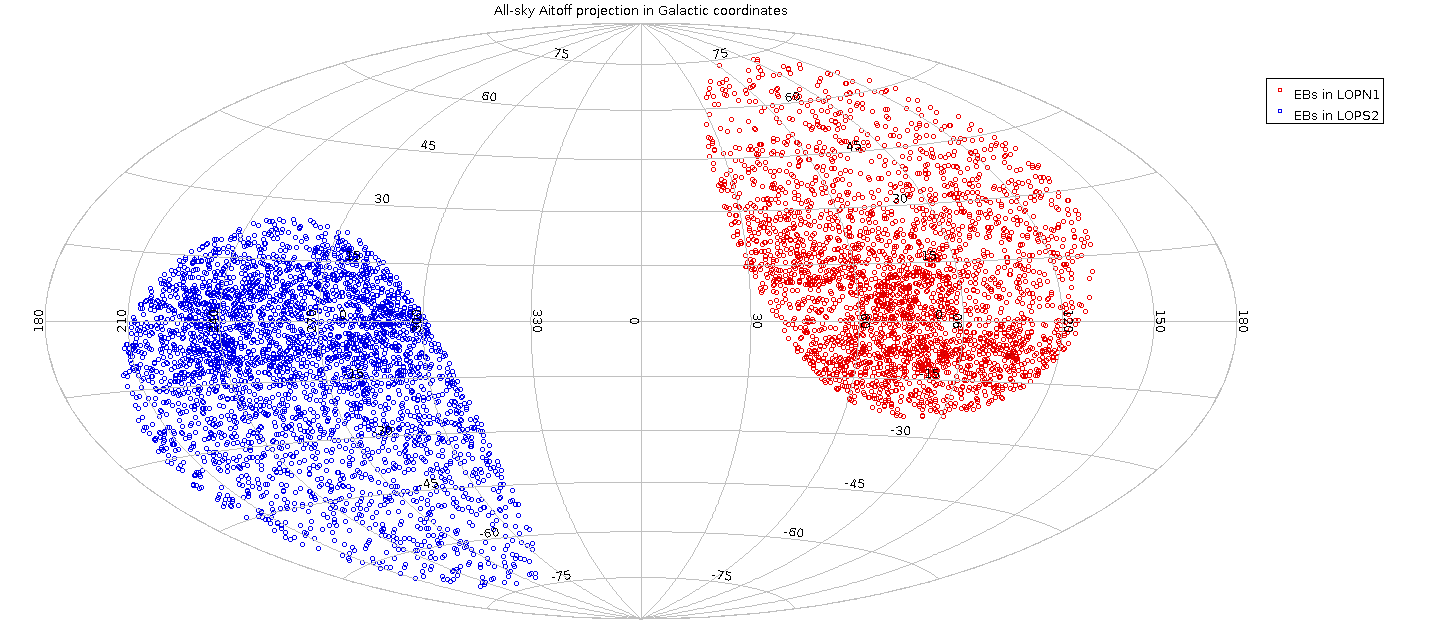
\includegraphics[scale=0.35]{EB_aitoff.png}
\caption{Sky map of eclipsing binaries in Galactic coordinates }
\label{fig:All-sky map of eclipsing binaries}
\end{figure}


\begin{comment}
\begin{figure}[H]
\centering
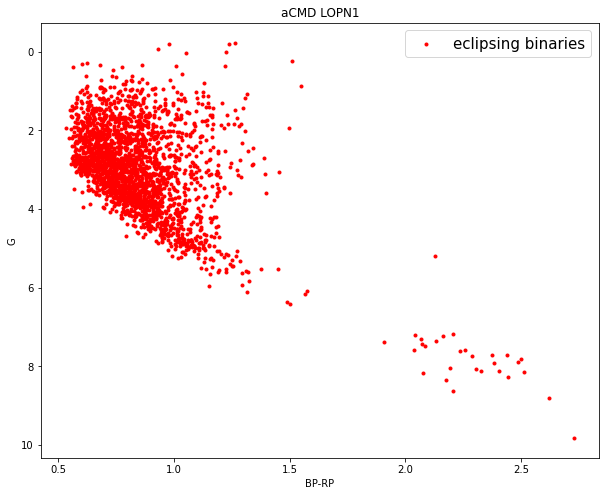
\includegraphics[scale=0.5]{eb_cmd.png}
\caption{Absolute CMD corrected for extinction for the eclipsing binaries in LOPN1}
\label{fig:Absolute CMD corrected for extinction for the eclipsing binaries in LOPN1}
\end{figure}


\begin{figure}[H]
\centering
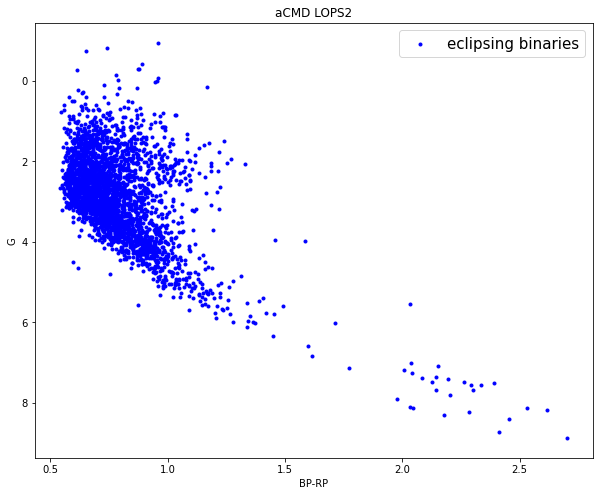
\includegraphics[scale=0.5]{eb2_cmd.png}
\caption{Absolute CMD corrected for extinction for the eclipsing binaries in LOPS2}
\label{fig:Absolute CMD corrected for extinction for the eclipsing binaries in LOPS2}
\end{figure}
\end{comment}

\begin{figure}[H]
\centering
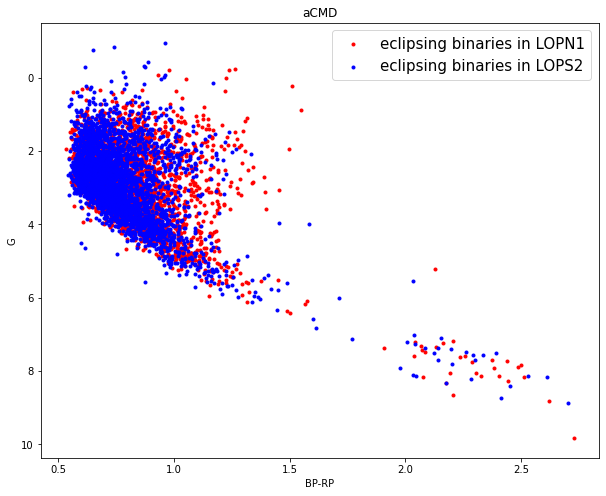
\includegraphics[scale=0.5]{eb_acmd.png}
\caption{Absolute CMD corrected for extinction for the total sample of eclipsing binaries in PIC}
\label{fig:Absolute CMD corrected for extinction for the total sample of eclipsing binaries in PIC}
\end{figure}


\begin{figure}[H]
\centering
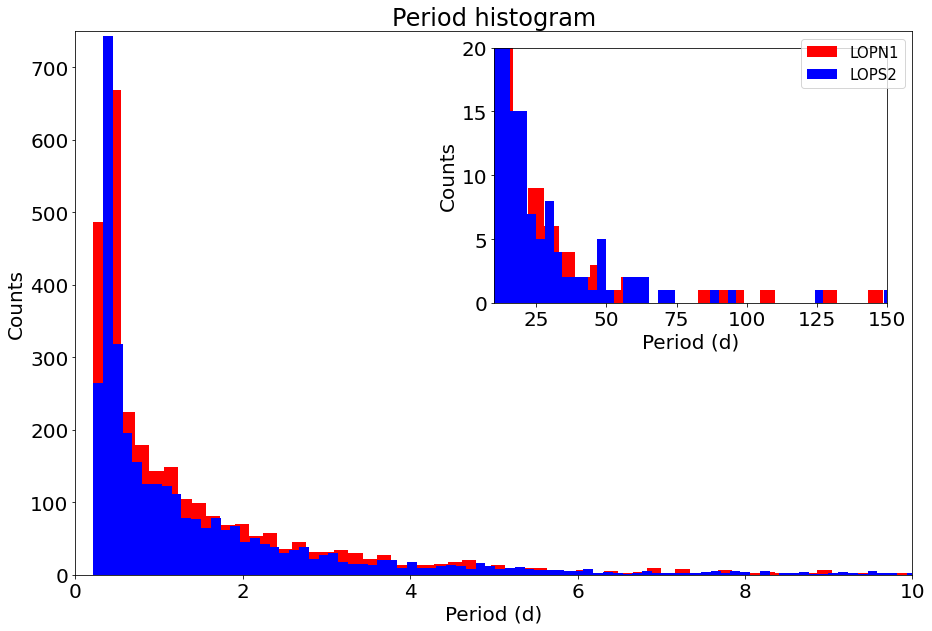
\includegraphics[scale=0.35]{periodhisto_eb.png}
\caption{Distribution of the orbital periods of the PIC eclipsing binaries. }
\label{fig:periodhisto_eb}
\end{figure}




\begin{figure}[H]
\centering
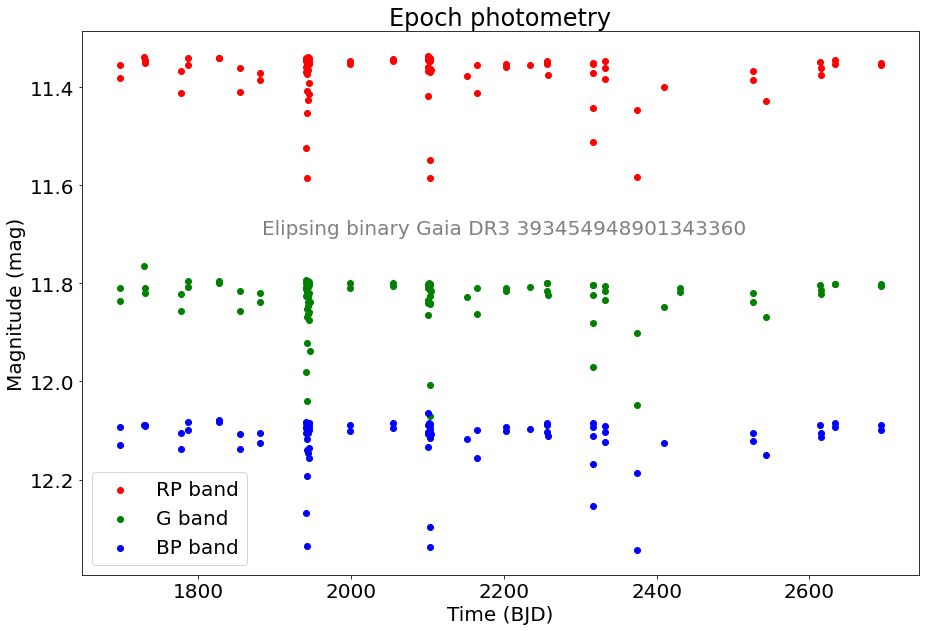
\includegraphics[scale=0.35]{eb1.png}
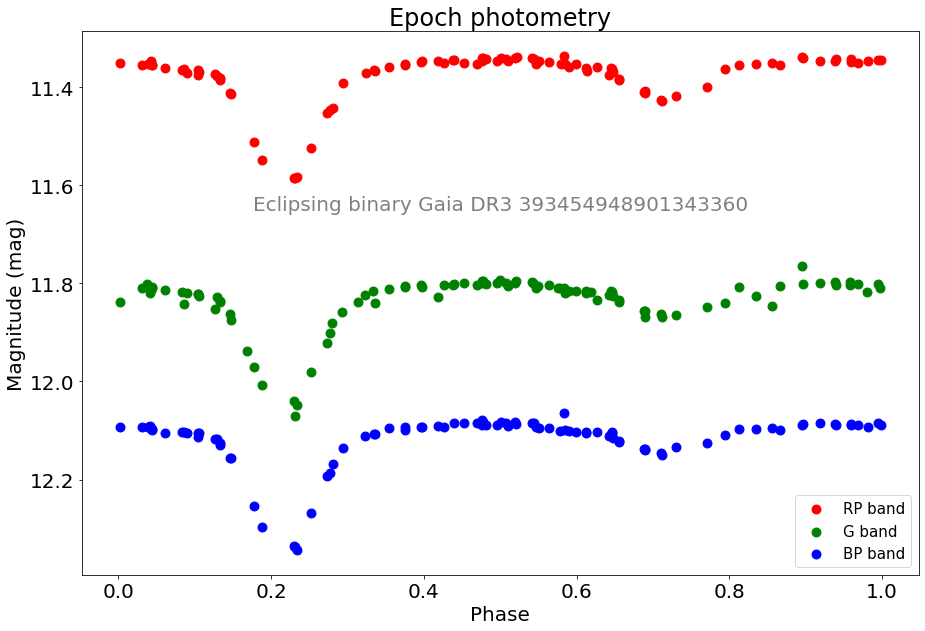
\includegraphics[scale=0.35]{eb2.png}
\caption{Light curve of the eclipsing binary Gaia DR3 393454948901343360, in the time domain (top) and folded according to the orbital period P = 1.72 d (bottom).}
\label{fig:binary}
\end{figure}




\newpage


\section{Short timescale variables}

The PLATO Input Catalogue counts over seven thousands objects that exhibit very fast variability, with periods ranging from 20 minutes to a day \footnote{Sources with periods between 0.5 and 1 d are considered ‘extended’ short-
timescale variables.} and amplitudes ranking from a few millimagnitudes to a few magnitudes.
These short-timescale variable sources are classified as EW-type eclipsing binaries, post-common envelope binaries (PCEB), cataclysmic variables (CV), RRab Lyrae stars, solar-like variables (rotational modulation, BY Draconis, RS Canum Venaticorum stars) and Main Sequence oscillators such as $\delta$ Scuti stars.

Gaia provides an exceptional opportunity for comprehensive fast-variability studies over the whole sky, thanks to its fast cadence time sampling in G band and its high photometric precision.

\cite{Roelens_2018} identified the candidates to be included in the Gaia DR3 \textit{short\_timescale} SOS module via variogram analysis; this method quantifies the magnitude variations between photometric measurements as a function of the time lag between them and defines a detection threshold above which the variability is significant enough at time lags shorter than 12 h.



%Gaia per-CCD photometric time series in G band + Gaia short-timescale analysis also made use of the filtered magnitude time series in G FoV (i.e. averaging the G CCD measurements within one FoV transit), G BP , and G RP
%on-board G measurements occur in groups of (most often) nine CCD observations (one every 4.85 s), one such group being referred to as a field-of-view (FoV) transit. Often, two or more FoV transits are repeated, with time intervals of 1h46min or 4h14min between successive FoVs, following the Gaia scanning law

%Variability statistical test: scatter in the G per-CCD points of each FoV transit is greater than a specific significance level.

The all-sky map in Aitoff projection and Galactic coordinates of the PLATO Input Catalogue's short timescale variables is shown in figure \ref{fig:All-sky map of short-time variables}, while fig. \ref{fig:short_acmd} displays the observational Hertzsprung-Russell diagram corrected for extinction.
In figures \ref{fig:freq_short} and \ref{fig:short_period} the amplitude-frequency plot and the periods distribution can be observed.
The lightcurves in time and phase domain of the short-timescale eclipsing binary Gaia DR3  4594961454434214144 are reported in figure \ref{fig:short_time}.


\begin{figure}[H]
\centering
\includegraphics[scale=0.35]{short_aitoff.png}
\caption{Sky map of short-time variables in Galactic coordinates }
\label{fig:All-sky map of short-time variables}
\end{figure}

\begin{comment}
\begin{figure}[H]
\centering
\includegraphics[scale=0.5]{short_cmd.png}
\caption{Absolute CMD corrected for extinction for short timescale variables in LOPN1}
\label{fig:Absolute CMD corrected for extinction for the short timescale variables in LOPN1}
\end{figure}


\begin{figure}[H]
\centering
\includegraphics[scale=0.5]{short2_cmd.png}
\caption{Absolute CMD corrected for extinction for short timescale variables in LOPS2}
\label{fig:Absolute CMD corrected for extinction for the short timescale variables in LOPS2}
\end{figure}
\end{comment}

\begin{figure}[H]
\centering
\includegraphics[scale=0.5]{short_acmd.png}
\caption{Absolute CMD corrected for extinction for the total sample of short timescale variables in PIC}
\label{fig:short_acmd}
\end{figure}


\begin{figure}[H]
\centering
\includegraphics[scale=0.35]{freq_short.png}
\caption{Frequency-amplitude distribution for the short-timescale variables in PIC.}
\label{fig:freq_short}
\end{figure}


\begin{figure}[H]
\centering
\includegraphics[scale=0.35]{short_period.png}
\caption{Period distribution for the short-timescale variables in PIC.}
\label{fig:short_period}
\end{figure}



\begin{figure}[H]
\centering
\includegraphics[scale=0.35]{short_epoch.png}
\includegraphics[scale=0.35]{short_fold.png}
\caption{Light curve for the short-timescale binary star Gaia DR3 4594961454434214144 in the time domain (top) and in the phase domain (bottom).}
\label{fig:short_time}
\end{figure}



\newpage

\section{Long period variables}


Long period variables (LPV) are typically stars from the asymptotic giant branch (AGB) and the red giant branch (RGB) who show large variability amplitudes, in particular in the visual range, and periods ranging from a few tens of days to 1000 d \parencite{refId9}.\\
The Gaia DR3 catalogue contains 1 720 558 LPV candidates, but only one of them is included in the all-sky PLATO Input Catalogue.\\
This source, identified as Gaia DR3 3005222633152619904 and EM* AS 119, is a cool, carbon-rich T Tauri giant star of spectral type B3IV[e].\\
Its time series in the Gaia photometric bands and its phase-folded light curve according to the tentative period P = 100 d are reported in figure \ref{fig:lpv}.

\begin{figure}[H]
\centering
\includegraphics[scale=0.35]{lpv_epoch.png}
\includegraphics[scale=0.35]{lpv_phase.png}
\caption{Time series (top) and phase-folded lightcurve (bottom) in the G, $G_{BP}$ and $G_{RP}$ bands for the long period variable Gaia DR3 3005222633152619904. }
\label{fig:lpv}
\end{figure}





\newpage

\section{Cepheids}

Cepheids are a class of periodic variable objects marked by a strong correlation between their absolute magnitude and period, which makes them standard candles to measure extra galactic distances, similarly to RR Lyrae stars.
They can be classified as classical Cepheids ($\delta$ Cep), type II Cepheids (T2CEPs) and anomalous Cepheids (ACEPs).\\
The first family is the most populated and significant one: $\delta$ Cep are typically luminous, young (50-500 Myr) and massive (M $\approx$ 3–11 $M\odot$) stars, that can be used to test stellar evolution models, trace the metallicity gradient of the Milky Way, and model the galactic thin disc \parencite{ripepi}.

Among 15 000 Cepheids included in the Gaia DR3 variable objects collection, only one of them figures in the PLATO Input Catalogue: this source is the $\delta$ Cep Gaia DR3 4301612233202961024, whose first overtone pulsation period is P = 0.219 d.
Its photometric time series and phase-folded lightcurve are displayed in figure \ref{fig:cep}.

\begin{figure}[H]
\centering
\includegraphics[scale=0.35]{cep_epoch.png}
\includegraphics[scale=0.35]{cep_fold.png}
\caption{Time series (top) and phase-folded lightcurve (bottom) in the G, $G_{BP}$ and $G_{RP}$ bands for the Cepheid Gaia DR3 4301612233202961024 over the first overtone period P = 0.219 d.}
\label{fig:cep}
\end{figure}




\chapter{Cross-matching catalogues}
\section{Section Title}



\parencite{https://doi.org/10.48550/arxiv.2207.01946}









\chapter{Conclusion}


% \parencite{Montalto_2021}, \parencite{Nascimbeni_2022}\parencite{Eyer} \parencite{Rimoldini} \parencite{Panahi_2022} \parencite{https://doi.org/10.48550/arxiv.2207.01946} \parencite{https://doi.org/10.48550/arxiv.2208.00211} \parencite{2016} \parencite{refId0} \parencite{refId1} \parencite{refId2} \parencite{refId3} \parencite{refId4} \parencite{refId5} \parencite{refId6} \parencite{refId7} \parencite{refId8}\parencite{refId9} \parencite{mowlavi2022gaia} \parencite{Roelens_2018}


\appendix
\chapter{Appendix Title}
Appendix 

% in this work, the term transit indicates the crossing of the entire focal plane by a given source.
\singlespacing
\printbibliography
\end{document}
